
%% bare_jrnl_compsoc.tex
%% V1.4b
%% 2015/08/26
%% by Michael Shell
%% See:
%% http://www.michaelshell.org/
%% for current contact information.
%%
%% This is a skeleton file demonstrating the use of IEEEtran.cls
%% (requires IEEEtran.cls version 1.8b or later) with an IEEE
%% Computer Society journal paper.
%%
%% Support sites:
%% http://www.michaelshell.org/tex/ieeetran/
%% http://www.ctan.org/pkg/ieeetran
%% and
%% http://www.ieee.org/

%%*************************************************************************
%% Legal Notice:
%% This code is offered as-is without any warranty either expressed or
%% implied; without even the implied warranty of MERCHANTABILITY or
%% FITNESS FOR A PARTICULAR PURPOSE!
%% User assumes all risk.
%% In no event shall the IEEE or any contributor to this code be liable for
%% any damages or losses, including, but not limited to, incidental,
%% consequential, or any other damages, resulting from the use or misuse
%% of any information contained here.
%%
%% All comments are the opinions of their respective authors and are not
%% necessarily endorsed by the IEEE.
%%
%% This work is distributed under the LaTeX Project Public License (LPPL)
%% ( http://www.latex-project.org/ ) version 1.3, and may be freely used,
%% distributed and modified. A copy of the LPPL, version 1.3, is included
%% in the base LaTeX documentation of all distributions of LaTeX released
%% 2003/12/01 or later.
%% Retain all contribution notices and credits.
%% ** Modified files should be clearly indicated as such, including  **
%% ** renaming them and changing author support contact information. **
%%*************************************************************************


% *** Authors should verify (and, if needed, correct) their LaTeX system  ***
% *** with the testflow diagnostic prior to trusting their LaTeX platform ***
% *** with production work. The IEEE's font choices and paper sizes can   ***
% *** trigger bugs that do not appear when using other class files.       ***                          ***
% The testflow support page is at:
% http://www.michaelshell.org/tex/testflow/


\documentclass[10pt,journal,compsoc]{IEEEtran}
%
% If IEEEtran.cls has not been installed into the LaTeX system files,
% manually specify the path to it like:
% \documentclass[10pt,journal,compsoc]{../sty/IEEEtran}





% Some very useful LaTeX packages include:
% (uncomment the ones you want to load)


% *** MISC UTILITY PACKAGES ***
%
%\usepackage{ifpdf}
% Heiko Oberdiek's ifpdf.sty is very useful if you need conditional
% compilation based on whether the output is pdf or dvi.
% usage:
% \ifpdf
%   % pdf code
% \else
%   % dvi code
% \fi
% The latest version of ifpdf.sty can be obtained from:
% http://www.ctan.org/pkg/ifpdf
% Also, note that IEEEtran.cls V1.7 and later provides a builtin
% \ifCLASSINFOpdf conditional that works the same way.
% When switching from latex to pdflatex and vice-versa, the compiler may
% have to be run twice to clear warning/error messages.






% *** CITATION PACKAGES ***
%
\ifCLASSOPTIONcompsoc
  % IEEE Computer Society needs nocompress option
  % requires cite.sty v4.0 or later (November 2003)
  \usepackage[nocompress]{cite}
\else
  % normal IEEE
  \usepackage{cite}
\fi
% cite.sty was written by Donald Arseneau
% V1.6 and later of IEEEtran pre-defines the format of the cite.sty package
% \cite{} output to follow that of the IEEE. Loading the cite package will
% result in citation numbers being automatically sorted and properly
% "compressed/ranged". e.g., [1], [9], [2], [7], [5], [6] without using
% cite.sty will become [1], [2], [5]--[7], [9] using cite.sty. cite.sty's
% \cite will automatically add leading space, if needed. Use cite.sty's
% noadjust option (cite.sty V3.8 and later) if you want to turn this off
% such as if a citation ever needs to be enclosed in parenthesis.
% cite.sty is already installed on most LaTeX systems. Be sure and use
% version 5.0 (2009-03-20) and later if using hyperref.sty.
% The latest version can be obtained at:
% http://www.ctan.org/pkg/cite
% The documentation is contained in the cite.sty file itself.
%
% Note that some packages require special options to format as the Computer
% Society requires. In particular, Computer Society  papers do not use
% compressed citation ranges as is done in typical IEEE papers
% (e.g., [1]-[4]). Instead, they list every citation separately in order
% (e.g., [1], [2], [3], [4]). To get the latter we need to load the cite
% package with the nocompress option which is supported by cite.sty v4.0
% and later. Note also the use of a CLASSOPTION conditional provided by
% IEEEtran.cls V1.7 and later.





% *** GRAPHICS RELATED PACKAGES ***
%
\ifCLASSINFOpdf
  % \usepackage[pdftex]{graphicx}
  % declare the path(s) where your graphic files are
  % \graphicspath{{../pdf/}{../jpeg/}}
  % and their extensions so you won't have to specify these with
  % every instance of \includegraphics
  % \DeclareGraphicsExtensions{.pdf,.jpeg,.png}
\else
  % or other class option (dvipsone, dvipdf, if not using dvips). graphicx
  % will default to the driver specified in the system graphics.cfg if no
  % driver is specified.
  % \usepackage[dvips]{graphicx}
  % declare the path(s) where your graphic files are
  % \graphicspath{{../eps/}}
  % and their extensions so you won't have to specify these with
  % every instance of \includegraphics
  % \DeclareGraphicsExtensions{.eps}
\fi
% graphicx was written by David Carlisle and Sebastian Rahtz. It is
% required if you want graphics, photos, etc. graphicx.sty is already
% installed on most LaTeX systems. The latest version and documentation
% can be obtained at:
% http://www.ctan.org/pkg/graphicx
% Another good source of documentation is "Using Imported Graphics in
% LaTeX2e" by Keith Reckdahl which can be found at:
% http://www.ctan.org/pkg/epslatex
%
% latex, and pdflatex in dvi mode, support graphics in encapsulated
% postscript (.eps) format. pdflatex in pdf mode supports graphics
% in .pdf, .jpeg, .png and .mps (metapost) formats. Users should ensure
% that all non-photo figures use a vector format (.eps, .pdf, .mps) and
% not a bitmapped formats (.jpeg, .png). The IEEE frowns on bitmapped formats
% which can result in "jaggedy"/blurry rendering of lines and letters as
% well as large increases in file sizes.
%
% You can find documentation about the pdfTeX application at:
% http://www.tug.org/applications/pdftex






% *** MATH PACKAGES ***
%
%\usepackage{amsmath}
% A popular package from the American Mathematical Society that provides
% many useful and powerful commands for dealing with mathematics.
%
% Note that the amsmath package sets \interdisplaylinepenalty to 10000
% thus preventing page breaks from occurring within multiline equations. Use:
%\interdisplaylinepenalty=2500
% after loading amsmath to restore such page breaks as IEEEtran.cls normally
% does. amsmath.sty is already installed on most LaTeX systems. The latest
% version and documentation can be obtained at:
% http://www.ctan.org/pkg/amsmath





% *** SPECIALIZED LIST PACKAGES ***
%
%\usepackage{algorithmic}
% algorithmic.sty was written by Peter Williams and Rogerio Brito.
% This package provides an algorithmic environment fo describing algorithms.
% You can use the algorithmic environment in-text or within a figure
% environment to provide for a floating algorithm. Do NOT use the algorithm
% floating environment provided by algorithm.sty (by the same authors) or
% algorithm2e.sty (by Christophe Fiorio) as the IEEE does not use dedicated
% algorithm float types and packages that provide these will not provide
% correct IEEE style captions. The latest version and documentation of
% algorithmic.sty can be obtained at:
% http://www.ctan.org/pkg/algorithms
% Also of interest may be the (relatively newer and more customizable)
% algorithmicx.sty package by Szasz Janos:
% http://www.ctan.org/pkg/algorithmicx




% *** ALIGNMENT PACKAGES ***
%
%\usepackage{array}
% Frank Mittelbach's and David Carlisle's array.sty patches and improves
% the standard LaTeX2e array and tabular environments to provide better
% appearance and additional user controls. As the default LaTeX2e table
% generation code is lacking to the point of almost being broken with
% respect to the quality of the end results, all users are strongly
% advised to use an enhanced (at the very least that provided by array.sty)
% set of table tools. array.sty is already installed on most systems. The
% latest version and documentation can be obtained at:
% http://www.ctan.org/pkg/array


% IEEEtran contains the IEEEeqnarray family of commands that can be used to
% generate multiline equations as well as matrices, tables, etc., of high
% quality.




% *** SUBFIGURE PACKAGES ***
%\ifCLASSOPTIONcompsoc
%  \usepackage[caption=false,font=footnotesize,labelfont=sf,textfont=sf]{subfig}
%\else
%  \usepackage[caption=false,font=footnotesize]{subfig}
%\fi
% subfig.sty, written by Steven Douglas Cochran, is the modern replacement
% for subfigure.sty, the latter of which is no longer maintained and is
% incompatible with some LaTeX packages including fixltx2e. However,
% subfig.sty requires and automatically loads Axel Sommerfeldt's caption.sty
% which will override IEEEtran.cls' handling of captions and this will result
% in non-IEEE style figure/table captions. To prevent this problem, be sure
% and invoke subfig.sty's "caption=false" package option (available since
% subfig.sty version 1.3, 2005/06/28) as this is will preserve IEEEtran.cls
% handling of captions.
% Note that the Computer Society format requires a sans serif font rather
% than the serif font used in traditional IEEE formatting and thus the need
% to invoke different subfig.sty package options depending on whether
% compsoc mode has been enabled.
%
% The latest version and documentation of subfig.sty can be obtained at:
% http://www.ctan.org/pkg/subfig




% *** FLOAT PACKAGES ***
%
%\usepackage{fixltx2e}
% fixltx2e, the successor to the earlier fix2col.sty, was written by
% Frank Mittelbach and David Carlisle. This package corrects a few problems
% in the LaTeX2e kernel, the most notable of which is that in current
% LaTeX2e releases, the ordering of single and double column floats is not
% guaranteed to be preserved. Thus, an unpatched LaTeX2e can allow a
% single column figure to be placed prior to an earlier double column
% figure.
% Be aware that LaTeX2e kernels dated 2015 and later have fixltx2e.sty's
% corrections already built into the system in which case a warning will
% be issued if an attempt is made to load fixltx2e.sty as it is no longer
% needed.
% The latest version and documentation can be found at:
% http://www.ctan.org/pkg/fixltx2e


%\usepackage{stfloats}
% stfloats.sty was written by Sigitas Tolusis. This package gives LaTeX2e
% the ability to do double column floats at the bottom of the page as well
% as the top. (e.g., "\begin{figure*}[!b]" is not normally possible in
% LaTeX2e). It also provides a command:
%\fnbelowfloat
% to enable the placement of footnotes below bottom floats (the standard
% LaTeX2e kernel puts them above bottom floats). This is an invasive package
% which rewrites many portions of the LaTeX2e float routines. It may not work
% with other packages that modify the LaTeX2e float routines. The latest
% version and documentation can be obtained at:
% http://www.ctan.org/pkg/stfloats
% Do not use the stfloats baselinefloat ability as the IEEE does not allow
% \baselineskip to stretch. Authors submitting work to the IEEE should note
% that the IEEE rarely uses double column equations and that authors should try
% to avoid such use. Do not be tempted to use the cuted.sty or midfloat.sty
% packages (also by Sigitas Tolusis) as the IEEE does not format its papers in
% such ways.
% Do not attempt to use stfloats with fixltx2e as they are incompatible.
% Instead, use Morten Hogholm'a dblfloatfix which combines the features
% of both fixltx2e and stfloats:
%
% \usepackage{dblfloatfix}
% The latest version can be found at:
% http://www.ctan.org/pkg/dblfloatfix




%\ifCLASSOPTIONcaptionsoff
%  \usepackage[nomarkers]{endfloat}
% \let\MYoriglatexcaption\caption
% \renewcommand{\caption}[2][\relax]{\MYoriglatexcaption[#2]{#2}}
%\fi
% endfloat.sty was written by James Darrell McCauley, Jeff Goldberg and
% Axel Sommerfeldt. This package may be useful when used in conjunction with
% IEEEtran.cls'  captionsoff option. Some IEEE journals/societies require that
% submissions have lists of figures/tables at the end of the paper and that
% figures/tables without any captions are placed on a page by themselves at
% the end of the document. If needed, the draftcls IEEEtran class option or
% \CLASSINPUTbaselinestretch interface can be used to increase the line
% spacing as well. Be sure and use the nomarkers option of endfloat to
% prevent endfloat from "marking" where the figures would have been placed
% in the text. The two hack lines of code above are a slight modification of
% that suggested by in the endfloat docs (section 8.4.1) to ensure that
% the full captions always appear in the list of figures/tables - even if
% the user used the short optional argument of \caption[]{}.
% IEEE papers do not typically make use of \caption[]'s optional argument,
% so this should not be an issue. A similar trick can be used to disable
% captions of packages such as subfig.sty that lack options to turn off
% the subcaptions:
% For subfig.sty:
% \let\MYorigsubfloat\subfloat
% \renewcommand{\subfloat}[2][\relax]{\MYorigsubfloat[]{#2}}
% However, the above trick will not work if both optional arguments of
% the \subfloat command are used. Furthermore, there needs to be a
% description of each subfigure *somewhere* and endfloat does not add
% subfigure captions to its list of figures. Thus, the best approach is to
% avoid the use of subfigure captions (many IEEE journals avoid them anyway)
% and instead reference/explain all the subfigures within the main caption.
% The latest version of endfloat.sty and its documentation can obtained at:
% http://www.ctan.org/pkg/endfloat
%
% The IEEEtran \ifCLASSOPTIONcaptionsoff conditional can also be used
% later in the document, say, to conditionally put the References on a
% page by themselves.




% *** PDF, URL AND HYPERLINK PACKAGES ***
%
%\usepackage{url}
% url.sty was written by Donald Arseneau. It provides better support for
% handling and breaking URLs. url.sty is already installed on most LaTeX
% systems. The latest version and documentation can be obtained at:
% http://www.ctan.org/pkg/url
% Basically, \url{my_url_here}.





% *** Do not adjust lengths that control margins, column widths, etc. ***
% *** Do not use packages that alter fonts (such as pslatex).         ***
% There should be no need to do such things with IEEEtran.cls V1.6 and later.
% (Unless specifically asked to do so by the journal or conference you plan
% to submit to, of course. )


% correct bad hyphenation here
\hyphenation{op-tical net-works semi-conduc-tor}

\usepackage{graphicx} % This is used to load the crest in the title page
\usepackage{subfigure}
%%%\usepackage{subfig}
\usepackage{algorithmic}
\usepackage{algorithm}
\usepackage{url}
\usepackage{times}
\usepackage{subfigure}
\usepackage{graphicx,epstopdf}
%\usepackage{latexsym}
%\usepackage{amsthm,amssymb}
%\usepackage{showkeys}
\usepackage{xcolor}
\usepackage{balance}
\usepackage{cite}
\usepackage[english]{babel}

% duan
\usepackage{xspace}

\newcommand{\spara}[1]{\smallskip\noindent{\bf #1}}
\newcommand{\eat}[1]{}
\newcommand{\squishlist}{
 \begin{list}{$\bullet$}
  {  \setlength{\itemsep}{0pt}
     \setlength{\parsep}{3pt}
     \setlength{\topsep}{3pt}
     \setlength{\partopsep}{0pt}
     \setlength{\leftmargin}{2em}
     \setlength{\labelwidth}{1.5em}
     \setlength{\labelsep}{0.5em}
} }
\newcommand{\squishlisttight}{
 \begin{list}{$\bullet$}
  { \setlength{\itemsep}{0pt}
    \setlength{\parsep}{0pt}
    \setlength{\topsep}{0pt}
    \setlength{\partopsep}{0pt}
    \setlength{\leftmargin}{2em}
    \setlength{\labelwidth}{1.5em}
    \setlength{\labelsep}{0.5em}
} }

\newcommand{\squishdesc}{
 \begin{list}{}
  {  \setlength{\itemsep}{0pt}
     \setlength{\parsep}{3pt}
     \setlength{\topsep}{3pt}
     \setlength{\partopsep}{0pt}
     \setlength{\leftmargin}{1em}
     \setlength{\labelwidth}{1.5em}
     \setlength{\labelsep}{0.5em}
} }

\newcommand{\squishend}{
  \end{list}
}
\newcommand{\sttab}{\rule{0pt}{8pt}\\[-3ex]}
\newcounter{ccc}
\newcommand{\bcc}{\setcounter{ccc}{1}\theccc.}
\newcommand{\icc}{\addtocounter{ccc}{1}\theccc.}
\newcommand{\myhrule}{\rule[.5pt]{\hsize}{.5pt}}
\newcommand{\mat}[2]{{\begin{tabbing}\hspace{#1}\=\+\kill #2\end{tabbing}}}
\newcommand{\stitle}[1]{\vspace{0.5ex}\noindent{\bf #1}}
\newcommand{\etitle}[1]{\vspace{0.5ex}\noindent{\em \underline{#1}}}
\newcommand{\marked}[1]{\textcolor{red}{#1}}
\newcommand{\markedb}[1]{\textcolor{blue}{#1}}

%%%%%%%%%% symbols of methods and datasets  by duan 2015-07-13
\newcommand{\DBLP}{{\sf DBLP}\xspace}
\newcommand{\SVD}{{\sf SVD}\xspace}
\newcommand{\NMF}{{\sf NMF}\xspace }
\newcommand{\Node}{{\sf NMF(Node)}\xspace}
\newcommand{\Edge}{{\sf NMF(Edge)}\xspace}
\newcommand{\Biased}{{\sf NMF(Biased)}\xspace}
\newcommand{\Aa}{{\sf AA}\xspace }
\newcommand{\Adamic}{{\sf Adamic/Adar (AA)}\xspace}
\newcommand{\Katz}{{\sf Katz}\xspace}
\newcommand{\BIGCLAM}{{\sf BIGCLAM}\xspace}
\newcommand{\CAMBN}{{\sf Cluster Affiliation Model for Big Networks (BIGCLAM)}\xspace}
\newcommand{\Digg}{{\sf Digg}\xspace}
\newcommand{\YouTube}{{\sf YouTube}\xspace}
\newcommand{\Flickr}{{\sf Flickr}\xspace}
\newcommand{\Wikipedia}{{\sf Wikipedia}\xspace}
\newcommand{\Twitter}{{\sf Twitter}\xspace}
\newcommand{\Friendster}{{\sf Friendster}\xspace}
\newcommand{\Nodep}{{\sf NMF(Node+)}\xspace}
\newcommand{\Edgep}{{\sf NMF(Edge+)}\xspace}
\newcommand{\Biasedp}{{\sf NMF(Biased+)}\xspace}



\newtheorem{definition}{Definition}

\newtheorem{observation}{Observation}
\newtheorem{lemma}{Lemma}
\newtheorem{prop}{Proposition}
\newtheorem{theorem}{Theorem}
\newtheorem{problem}{Problem}
\newtheorem{corollary}{Corollary}
\newtheorem{property}{Property}
\newcommand{\lemmachar}{{\unskip\nobreak\hfil\penalty50\hskip1em\hbox{}%
\nobreak\hfil\rule{1.2ex}{1.4ex}\hfil%
\parfillskip=0pt \finalhyphendemerits=0 \par}}



%\newenvironment{proof}{{\bf Proof:}}{\lemmachar\par}


\newfont{\mycrnotice}{ptmr8t at 7pt}
\newfont{\myconfname}{ptmri8t at 7pt}
\let\crnotice\mycrnotice%
\let\confname\myconfname%




\begin{document}
%
% paper title
% Titles are generally capitalized except for words such as a, an, and, as,
% at, but, by, for, in, nor, of, on, or, the, to and up, which are usually
% not capitalized unless they are the first or last word of the title.
% Linebreaks \\ can be used within to get better formatting as desired.
% Do not put math or special symbols in the title.
\title{Scaling up Link Prediction with Ensembles}
\title{Scaling up Link Prediction with Sampling based Ensembles}
\title{Scaling up Link Prediction with Ensembles based on Sampling}
\title{Scaling up Link Prediction: an Ensemble Enabled Approach}
\title{Scaling up Link Prediction with Ensembles: Sampling with Sparsification}
\title{An Ensemble Approach to Scaling up Link Prediction}
\title{An Ensemble Approach to Link Prediction}
%
%
% author names and IEEE memberships
% note positions of commas and nonbreaking spaces ( ~ ) LaTeX will not break
% a structure at a ~ so this keeps an author's name from being broken across
% two lines.
% use \thanks{} to gain access to the first footnote area
% a separate \thanks must be used for each paragraph as LaTeX2e's \thanks
% was not built to handle multiple paragraphs
%
%
%\IEEEcompsocitemizethanks is a special \thanks that produces the bulleted
% lists the Computer Society journals use for "first footnote" author
% affiliations. Use \IEEEcompsocthanksitem which works much like \item
% for each affiliation group. When not in compsoc mode,
% \IEEEcompsocitemizethanks becomes like \thanks and
% \IEEEcompsocthanksitem becomes a line break with idention. This
% facilitates dual compilation, although admittedly the differences in the
% desired content of \author between the different types of papers makes a
% one-size-fits-all approach a daunting prospect. For instance, compsoc
% journal papers have the author affiliations above the "Manuscript
% received ..."  text while in non-compsoc journals this is reversed. Sigh.

\author{Liang~Duan,
        Shuai~Ma,
        Charu~Aggarwal,
        and~Jinpeng~Huai
\IEEEcompsocitemizethanks{\IEEEcompsocthanksitem L. Duan, S. Ma and J. Huai are
with the SKLSDE lab \& BDBC center, School of Computer Science and Engineering, Beihang University, China.\hfil\break
% note need leading \protect in front of \\ to get a newline within \thanks as
% \\ is fragile and will error, could use \hfil\break instead.
E-mail: \{duanliang, mashuai, hurenjun, huaijp\}@buaa.edu.cn
\IEEEcompsocthanksitem C. Aggarwal is with the IBM Thomas J. Watson Research Center, USA.\hfil\break
E-mail: charu@us.ibm.com}% <-this % stops an unwanted space
\thanks{Manuscript received XXX, 2016; revised XXX, 2016.}}

% note the % following the last \IEEEmembership and also \thanks -
% these prevent an unwanted space from occurring between the last author name
% and the end of the author line. i.e., if you had this:
%
% \author{....lastname \thanks{...} \thanks{...} }
%                     ^------------^------------^----Do not want these spaces!
%
% a space would be appended to the last name and could cause every name on that
% line to be shifted left slightly. This is one of those "LaTeX things". For
% instance, "\textbf{A} \textbf{B}" will typeset as "A B" not "AB". To get
% "AB" then you have to do: "\textbf{A}\textbf{B}"
% \thanks is no different in this regard, so shield the last } of each \thanks
% that ends a line with a % and do not let a space in before the next \thanks.
% Spaces after \IEEEmembership other than the last one are OK (and needed) as
% you are supposed to have spaces between the names. For what it is worth,
% this is a minor point as most people would not even notice if the said evil
% space somehow managed to creep in.



% The paper headers
\markboth{IEEE Transactions on Knowledge and Data Engineering,~Vol.~X, No.~X, May~2016}%
{Shell \MakeLowercase{\textit{et al.}}: Bare Demo of IEEEtran.cls for Computer Society Journals}
% The only time the second header will appear is for the odd numbered pages
% after the title page when using the twoside option.
%
% *** Note that you probably will NOT want to include the author's ***
% *** name in the headers of peer review papers.                   ***
% You can use \ifCLASSOPTIONpeerreview for conditional compilation here if
% you desire.



% The publisher's ID mark at the bottom of the page is less important with
% Computer Society journal papers as those publications place the marks
% outside of the main text columns and, therefore, unlike regular IEEE
% journals, the available text space is not reduced by their presence.
% If you want to put a publisher's ID mark on the page you can do it like
% this:
%\IEEEpubid{0000--0000/00\$00.00~\copyright~2015 IEEE}
% or like this to get the Computer Society new two part style.
%\IEEEpubid{\makebox[\columnwidth]{\hfill 0000--0000/00/\$00.00~\copyright~2015 IEEE}%
%\hspace{\columnsep}\makebox[\columnwidth]{Published by the IEEE Computer Society\hfill}}
% Remember, if you use this you must call \IEEEpubidadjcol in the second
% column for its text to clear the IEEEpubid mark (Computer Society jorunal
% papers don't need this extra clearance.)



% use for special paper notices
%\IEEEspecialpapernotice{(Invited Paper)}



% for Computer Society papers, we must declare the abstract and index terms
% PRIOR to the title within the \IEEEtitleabstractindextext IEEEtran
% command as these need to go into the title area created by \maketitle.
% As a general rule, do not put math, special symbols or citations
% in the abstract or keywords.
\IEEEtitleabstractindextext{%
\begin{abstract}
A network with $n$ nodes contains $O(n^2)$ possible links.
Even for networks of modest size, it is often difficult to evaluate
all pairwise possibilities for links in a meaningful way.
Furthermore, even though link prediction is closely related to
missing value estimation problems, such as collaborative filtering,
it is often difficult to use sophisticated models such as latent
factor methods because of their computational complexity over
very large networks. Due to this computational complexity, most
known link prediction methods are designed for {\em evaluating} the
link propensity over a {\em specified} subset of links, rather than
for performing a global search over the entire networks. In
practice,  however, it is essential to perform an exhaustive search over the
entire networks.  In this paper, we propose an ensemble enabled approach to scaling up link prediction,
which is able to decompose traditional link prediction problems into
subproblems of smaller size. These subproblems are each solved with
the use of latent factor models, which can be effectively
implemented over networks of modest size. Furthermore, the
ensemble enabled approach has several advantages in terms of
performance. \marked{Incorporating with some link prediction
characteristics, we optimize the ensemble approach by reducing the
sizes of subproblems without sacrificing prediction accuracy. }
 We show the advantage of using ensemble-based latent
factor models  with experiments on very large networks.
Experimental results demonstrate the effectiveness and scalability of our approach.
\end{abstract}

% Note that keywords are not normally used for peerreview papers.
\begin{IEEEkeywords}
Link Prediction, ensembles, networks, Big Data.
\end{IEEEkeywords}}


% make the title area
\maketitle


% To allow for easy dual compilation without having to reenter the
% abstract/keywords data, the \IEEEtitleabstractindextext text will
% not be used in maketitle, but will appear (i.e., to be "transported")
% here as \IEEEdisplaynontitleabstractindextext when the compsoc
% or transmag modes are not selected <OR> if conference mode is selected
% - because all conference papers position the abstract like regular
% papers do.
\IEEEdisplaynontitleabstractindextext
% \IEEEdisplaynontitleabstractindextext has no effect when using
% compsoc or transmag under a non-conference mode.



% For peer review papers, you can put extra information on the cover
% page as needed:
% \ifCLASSOPTIONpeerreview
% \begin{center} \bfseries EDICS Category: 3-BBND \end{center}
% \fi
%
% For peerreview papers, this IEEEtran command inserts a page break and
% creates the second title. It will be ignored for other modes.
\IEEEpeerreviewmaketitle


%%% Local Variables:
%%% mode: latex
%%% TeX-master: "gis18"
%%% End:

\section{introduction}
\label{sec-intro}


\textit{Trajectory tracking} \cite{Lange:Tracking} is a combination of \textit{position tracking} \cite{Wolfson:PositionTracking,Leonhardi:Comparison} and \textit{trajectory simplification} \cite{Lin:Cised,Zhang:Evaluation} in one routine, where \textit{position tracking} is an approach that lets the moving objects database (MOD) server know the current position of a moving object effectively and efficiently, that is, it achieves the desired accuracy of the location information on the server by transmitting as few messages as possible \cite{Leonhardi:Comparison}. Linear dead reckoning (\ldr) \cite{Wolfson:PositionTracking} is such a widely used position tracking method, which is essentially an agreement between a given moving object and a MOD server such that the server could infer the current, excepted position of the moving object whose distance to the actual position of the object is bounded by a user specified threshold;
%
and \textit{trajectory simplification} \cite{Lin:Cised,Zhang:Evaluation} is to approximate a fine trajectory with a coarse one (whose corresponding data points are a subset of the original one), such that the size of the trajectory is reduced under a constrain that the maximum distance of the former to the latter is bounded by a user specified threshold. 
%Linear simplification \cite{Lin:Cised,Zhang:Evaluation} is such an effective and efficient approach that is also widely used in practice.
%
Position tracking and trajectory simplification both are the fundamental technologies of trajectory management and they also share some common target and strategy, \ie, reduce the number of messages or the size of trajectory data by discarding some location information that seems not that important, hence, researchers are trying to combine them in one routine and make it be suitable to run in resource constraint devices.

The authors of \cite{Trajcevski:LDRH} find that the position tracking algorithm \ldr with some tiny modifications is applicable to both track the positions of a moving object and simplify the trajectory built out of these positions. The modified \ldr,  called \ldrh in \cite{Lange:Tracking}, is the first trajectory tracking algorithm that combines position tracking and trajectory simplification into one consistent process. It is concise and efficient, and is suitable for mobile devices. However, it suffers in effectiveness in terms of compression ratio and communication cost, due to the nature of \ldr. 
%
Then, a framework, named the generic remote trajectory simplification (GRTS) \cite{Lange:GRTS,Lange:Tracking}, is developed to improve the effectiveness of trajectory tracking by separate position tracking and trajectory simplification into two sub-processes, where the positions of a moving object is also tracked by \ldr, and these positions are temporarily saved in a buffer and then simplified by some third-party line simplification algorithm. Indeed, it is more effective than \ldrh at a cost of weakening the conciseness and efficiency of \ldrh.
%



\stitle{\todo{Motivations}.}

\ni(1) Trajectory track algorithms are supposed to run in resource-constraint mobile devices, thus, besides good performance of efficiency and effectiveness, they should also be simple and light, \ie having low time and space complexities, otherwise, they are not suitable to run in those mobile devices. In response to these requirements, \ldrh is light, simple and efficient, but not effective; and \grts is effective, but not efficient and light enough. That is, neither of them is the ideal solution for trajectory tracking.
%The emerging of one pass trajectory simplification algorithms. These algorithms can be integrated into grts, however, it is not a natural way to implement a one-pass trajectory tracking algorithm like this way. Acutually, one pass position tracking + one pass trajectory simplification = one pass and effective trajectory tracking algorithm......co-design, like LDRH, yet more effective.


\ni(2) The current works, \ie~\ldrh and \grts, only compress a trajectory or track a moving object in circular areas, \ie the moving object is supposed to locate in a circular taking the expected position of the object as the center. However, in practical, there is a need to track moving objects in other areas, such as strip or rectangular-like areas. \todo{examples and figures of areas,}





\stitle{\todo{Contributions}.}
To the end, we design ways for trajectory tracking in varied areas, including strip and combined areas, and provide three novel one-pass algorithms tracking moving objects effectively and efficiently. 

1. one-pass tracking moving object in circular, citt, effectively and efficiently.

2. one-pass tracking in strips using ped. sitt.
a way that customize region by sed and ped. and implement it in position tracking LDR and trajectory tracking framework GRTS. advantage...

3. one-pass tracking in combined areas using sed and ped. bitt.  
A one-pass trajectory tracking algorithm supporting sed and ped, by a combination cone intersection and sector intersection, \ie co-design of position tracking and trajectory simplification, effective and low time and space complexity, suitable running in resource constraint devices.

4. experiments

\stitle{{Organization}}.
The remainder of the paper is organized as follows:
Section \ref{sec-pre} introduces the basic concepts and the basic HMM method,
Section \ref{sec-method} presents our trajectory simplification aware map-matching method,
Section \ref{sec-exp} reports the experimental results of these methods, followed by related works in Section \ref{sec-related} and conclusion in Section \ref{sec-conclusion}.




\section{Latent Factor Model for Link Prediction}
\label{sec-NMF}
\marked{In this section, we first provide a link prediction method 
based on latent factor models. We then design an efficient method to 
search the possible links from $O(n^2)$ search space.}


We assume that $G=(N, A)$ is an undirected network (or graph) containing node set $N$ and
edge set $A$. The node set $N$ contains $n$ nodes and the edge set
$A$ contains $m$ edges. Furthermore, the $n \times n$ weight matrix
$W= [w_{ij}]_{n\times n}$ contains the weights of the edges in $A$.
The weight matrix is useful in representing the strengths of network
connections in  many real-world settings such as the number of
publications between a pair of co-authors in a bibliographic
network.  The matrix is sparse, and many its entries are 0, which could be
interpreted either as absence of links or as missing entries. While
we assume that an undirected network is available, the approach can
also be generalized to directed networks.
%
 The top-$k$ ranking problem for link prediction is formally stated as follows:

\begin{definition}
Given a network $G=(N, A)$ with node set $N$ and edge set $A$, the ranking problem for link
prediction is to determine the top-$k$ node-pair recommendations such that these node pairs are not included in $A$.
\end{definition}
Note that this problem definition requires us to consider the entire
search space of $O(n^2)$ possibilities, rather than a sample of the
node pairs in the network.

Latent factor models work by associating a low dimensional factor
with each row and column of the network. However, since link
prediction is (predominantly) studied only for undirected networks,
which have symmetric weight matrices, it suffices to associate an
$r$-dimensional latent factor $\overline{f_i}$ with the $i$th node
in the network. The value of $r$ is the {\em rank} of the
factorization. This is an issue, which we will discuss slightly
later.  The weight of a link between nodes $i$ and $j$ is defined by
the use of the dot product between the factors of nodes $i$ and $j$.
In other words, for the weight matrix $W= [w_{ij}]_{n\times n}$, we
would like to achieve the following:
\begin{equation}
w_{ij} \approx \overline{f_i} \cdot \overline{f_j}, \ \ \forall i, j
\in \{ 1, \ldots, n \} \label{factor}.
\end{equation}
This condition can be directly written in the matrix form. Let $F$ be an
$n \times r$ matrix, in which the $i$th row is the row vector
$\overline{f_i}$. Then, the above condition of
Equation~(\ref{factor}) can be written as follows:
\begin{equation}
W \approx F F^T.
\end{equation}


%Note that the diagonal entries of $W$ are 0, whereas any reasonable
%factorization $F F^T$ will always have non-zero diagonal entries
%with magnitudes  dependent on the node degrees.  To make the
%factorization more robust, we set each diagonal entry $w_{ii}$ to
%the sum of the weights of the edges  incident on it.
%\begin{equation}
%w_{ii}= \sum_{j \not=i} w_{ij}
%\end{equation}
%%The resulting matrix can  also be shown to be  positive
%%semi-definite, which ensures that an {\em exact} rank-$n$
%%factorization of $W$ into the form $F F^T$ always exists.
%The resulting matrix can also be shown to be nonnegative
%diagonally dominant symmetric, which ensures that an {\em exact}
%rank-$n$ factorization of $W$ into the form $F F^T$ always exists \cite{berman}.
%Of course, we are only interested in a rank-$r$ factorization ($r << n$),
%corresponding to dominant latent components,  because such a
%factorization helps in discovering {\em latent} edges.


An important question arises as to whether entries in the matrix $W$
corresponding to the absence of links should be treated as incomplete
entries or whether they should be treated as zero, with the possibility
of being incorrect. When latent factor models are used in
collaborative filtering, such entries are typically treated as
missing entries. However, unlike the absence of a rating, the
absence of a link is indeed useful information {\em in the
aggregate}, even though some node pairs have the propensity to form
links {\em in the future}. Therefore, we argue that, unlike
collaborative filtering, $W$ should be treated as a completely
specified matrix, but with noisy entries. Therefore, in the link
prediction problem, latent factor models should be viewed as a way
of {\em correcting} noisy entries with zero values, rather than
strictly as a missing value estimation problem.  Such assumptions
also simplify the algorithmic development of latent factor models
for link prediction. The idea here is that when we approximately
factorize $W$ into the form  $F F^T$, the positive values of entries in
$F F^T$ can be viewed as the {\em predictions} of  noisy 0-entries in
$W$.

A second important question arises as to the choice of the latent
factor model that must be used for prediction. There are many
choices available for factorizing an adjacency matrix, especially
when it is symmetric. Even a
straightforward diagonalization of the matrix provides a reasonable
factorization. We  choose {\em non-negative} matrix factorization (\NMF)
not only because of its interpretability advantages but also because
it facilitates the  $O(n^2)$ search phase of the prediction by
providing a non-negative and sparse representation for each node.

We would like to determine the matrix $F$ such that the Frobenius
norm of $( W - F F^T)$ is minimized.  This problem is referred to as
symmetric \NMF, and an efficient solution is proposed in
\cite{long}, where $F$ can be determined by starting with random
nonnegative entries in $(0, 1)$, and using the following
multiplicative update rule:
% {\bf Charu Note: Please check that this update works during implementation. NMF is sometimes unpredictable.}
%\begin{equation}
%F_{ij} \leftarrow  F_{ij} \frac{(W F)_{ij} }{(F F^T F)_{ij}}
%\end{equation}
\begin{equation}
\label{equation-update}
F_{ij} \leftarrow F_{ij} \left( 1 - \beta + \beta \frac{ \left(W F \right)_{ij} }{ \left(F F^T F \right)_{ij}} \right),
\end{equation}
in which $\beta$ is a constant in $( 0, 1]$ \cite{ding}.

\stitle{Discussions of computational complexity}. Let us examine the computational complexity of
the update Equation~(\ref{equation-update}).
The matrix $F F^T F$  can be fully materialized  with
$O(r^2 \cdot n)$ matrix multiplications, and the matrix $W F$ can be
computed in $O(m \cdot r)$ multiplications  by observing that the
sparse matrix $W$ has only $2m$ non-zero entries corresponding to the
number of edges. Therefore, each update takes $O(n
\cdot r^2 +m\cdot r )$ time.

This remains quite high for large networks, which motivates us to develop fast searching techniques to speed up the process.


\subsection{Efficient Top-$K$ Prediction Searching}
\label{sec-NMF-topk}

An advantage of the nonnegative factorization approach is that it
enables an efficient search phase, which is generally not possible
with most other link prediction methods. The value of
$\overline{f_i} \cdot \overline{f_j}$ in Equation~(\ref{factor}) provides a prediction value
for the links. The goal of the search phase is to return the top-$k$
links with the largest prediction values. In real-world settings, the matrix $F$ is
often nonnegative and sparse \cite{NMF-nature99}. This non-negativity and sparsity are
particularly useful in enabling an efficient approach. In order to
speed up the search, we define the notion of $\epsilon$-approximate
top-$k$ predictions, denoted as top-$(\epsilon, k)$ predictions.


\begin{definition}[top-$(\epsilon, k)$ predictions]
%A set $S$ of predicted links is a top-$(\epsilon, k)$ prediction, if
%the cardinality of $S$ is $k$, and the  $k$th best  value of
%$\overline{F_i} \cdot \overline{F_j}$ for a  link $(i, j) \in S$ is
%at most $\epsilon$ less than the   $k$th best value of
%$\overline{F_k} \cdot \overline{F_k}$ over any edge $(k , l)$ in the
%network.
A set $L$ of predicted links in a network is a top-$(\epsilon, k)$ prediction, if
the cardinality of $L$ is $k$, and the $k$-th best  value of
$\overline{f_i} \cdot \overline{f_j} $ for a link $(i, j) \in L$ is
at most $\epsilon$ less than the $k$-th best value of
$\overline{f_h} \cdot \overline{f_l}$ over any link $(h , l)$ in the
network.
\end{definition}
Intuitively, this definition allows a qualitative  tolerance of
$\epsilon$ in the top-$k$ returned links. Allowing such a tolerance
significantly helps in speeding up the search process by pruning
large portions of the search space, which is particularly important
in an $O(n^2)$ search space of link predictions.

The first step is to create a new $n \times r$ matrix $S$,
obtained by sorting the columns of $F$ in a descending order. An inverted list is
associated with each of the $r$ latent variables containing the node
identifiers  of $F$ arranged according to the sorted order of $S$. The
$r$ inverted lists can also be represented as an $n \times r$ matrix
$R$. Let the number of rows in the $p$-th column of $S$ ($p\in[1, r]$), for which
the value of $S_{ip}$ is greater than $\sqrt{\epsilon/r}$ be $f_p$, and for which the value of $S_{ip}$ is greater than 0 be $f'_p$, respectively.

Then the following nested loop is executed for each (say $p$-th) column of $S$:

%\vspace{-1ex}
\begin{tabbing}1. \hspace{5ex}\=
{\bf for} \= each $i=1$ to $f_p$ {\bf do}\\
2. \>\>{\bf for} \= each $j=i+1$ to $f'_p$ {\bf do}\\
3. \>\>\>{\bf if}\ \= $S_{ip} \cdot S_{jp} < \epsilon/r$ {\bf then}\\
4. \>\>\>\>break inner loop; \\
5. \>\>\> {\bf else} increase the score of node-pair $(R_{ip}, R_{jp})$ by \\
   \>\>\> \ \ \ \ \ \ an amount of $S_{ip} \cdot S_{jp}$\\
6. \>\> {\bf endfor}\\
7. \>{\bf endfor}
\end{tabbing}
%\vspace{-1ex}

This nested loop is designed to track the relevant subset of node
pairs from which one can determine the top-$(\epsilon, k)$
predictions.  The nested loop typically requires much less time than
$O(n^2)$ time because large portions of the search space are pruned.
First, depending on the value of $\epsilon$, the value of $f_p$ is
much less than $n$.  This is particularly true if many entries of
the factorized matrix $F$ are close to 0.  Furthermore, the inner
loop is often terminated early. The value of $\epsilon$ therefore
provides the user a way to set the tradeoff between accuracy and
efficiency. A hash-table is maintained which tracks all the pairs
$(R_{ip}, R_{jp})$ encountered so far in the nested loop. Because of
the pruning, the hash table usually needs to track a miniscule set
of the $O(n^2)$ node-pairs in order to determine the ones that truly satisfy the top-$(\epsilon, k)$ requirement. In the process, we exclude
the links which have already been represented with non-zero entries in $W$
because such links are always likely to have the largest prediction values,
which further reduces the searching space.

\eat{%%%%%%EAT
\begin{lemma}
For a $n \times r$ matrix $F$, the complexity of the top-$(\epsilon, k)$
prediction is $O(nn')$, where $n'$ is the number of entries of $F$
which are greater than $\sqrt{ \epsilon / r}$.
\end{lemma}
\begin{IEEEproof}
For the $p$th column of $F$, the {\bf if} statement in the nested loop
is executed $f_p ( 2n_p - f_p -1) / 2$ times. There are $r$ columns in $F$,
hence, the {\bf if} statement will be executed
$\sum_{p = 1}^{r} f_p ( 2n_p - f_p -1) / 2 $ times.
$\sum_{p = 1}^{r} f_p ( 2n_p - f_p -1) / 2 \leq n\sum_{p = 1}^{r}f_{p}$, and
$\sum_{p = 1}^{r} f_p$ is equal to the number $n'$. Therefore, the complexity of
top-$(\epsilon, k)$ prediction is $O(nn')$.
\end{IEEEproof} }

 It remains to show that this procedure does find a valid set of top-$(\epsilon,
k)$ link predictions. The reason that the procedure works correctly
and efficiently  is because of nonnegativity and sparsity. \marked{We next use an
example to illustrate how to search the top-$(\epsilon, k)$ link predictions based
on the above nested loop method.}

%%%%%%%%%%% example for top-k prediction
\vspace{2ex}
\noindent\marked{\begin{example}
\label{ex_top_k}
Given a $5 \times 3$ matrix $F$, we sort the three columns of $F$ in a
descending order to generate the matrix $S$ and store the corresponding
inverted indices in the matrix $R$, shown as follows:
\[\underbrace{
  \begin{bmatrix}
    0.7 & 0.3 & 0.7 \\
    0.5 & 0.7 & 0.9 \\
    0.4 & 1.1 & 0.7 \\
    0.0 & 0.8 & 0.0 \\
    0.5 & 0.0 & 0.1
  \end{bmatrix}}_{F}
  \Longrightarrow
  \underbrace{\begin{bmatrix}
    0.7 & 1.1 & 0.9 \\
    0.5 & 0.8 & 0.7 \\
    0.5 & 0.7 & 0.7 \\
    0.4 & 0.3 & 0.1 \\
    0.0 & 0.0 & 0.0
  \end{bmatrix}}_{S}
  \underbrace{\begin{bmatrix}
    1 & 3 & 2 \\
    2 & 4 & 1 \\
    5 & 2 & 3 \\
    3 & 1 & 5 \\
    4 & 5 & 4
  \end{bmatrix}}_{R}
\]
Assume that $\epsilon = 1$, then $\sqrt{ \epsilon / r} = 0.58$ and $\epsilon / r = 0.33$.
For $p = 1$ (resp. $p = 2$ and $p = 3$), we have ($f_1 = 1, f'_1 = 4$)
(resp. ($f_2 = 3, f'_2 = 4$) and ($f_3 = 3, f'_3 = 4$)) and only need to calculate
9 multiplications: ($S_{11} \cdot S_{21}$,
$S_{11} \cdot S_{31}$) (resp. ($S_{12} \cdot S_{22}$, $S_{12} \cdot S_{32}$, $S_{12} \cdot S_{42}$,
$S_{22} \cdot S_{32}$) and ($S_{13} \cdot S_{23}$, $S_{13} \cdot S_{33}$, $S_{23} \cdot S_{33}$))
rather than 75 multiplications for calculating $FF^T$ directly, thus pruning a large portion of
the search space. We then save the above values into corresponding node pairs,
\eg increase the score of node pair ($R_{11}, R_{21}$) by $S_{11} \cdot S_{21}$,
and finally return all node pairs that we encountered.
\end{example} }



\begin{prop}
\label{prop-valid-topk}
The nested loop method finds a valid set of top-$(\epsilon, k)$
predictions.
\end{prop}
\begin{IEEEproof}
The main part of the proof is to show that any dot product is
underestimated by at most  $\epsilon$. The aforementioned pseudo-code
containing the  nested loop is executed $r$ times, once for each
latent component. Therefore, it suffices to show that the
contribution of each nested loop is underestimated by at most
$\epsilon/r$. There are two sources of underestimation:
\begin{enumerate}
\item  The outer loop does not consider rows $i$ for which $S_{ip} <
\sqrt{\epsilon/r}$. This effectively prunes the products between
pairs $(i, j)$ for which both $S_{ip}$ and $S_{jp}$ are less
than $\sqrt{\epsilon/r}$ \marked{ since the matrix $S$ is sorted and $S_{ip} \geq S_{jp}$}.
Therefore, the underestimation because of
the ignoring of this pair is at most $\sqrt{\epsilon/r} \times
\sqrt{\epsilon/r} = \epsilon/r$.
\item The second case is when the inner loop is terminated early.
The early termination condition in this case is that the product is
at most $\epsilon/r$.
\end{enumerate}
Therefore, in both these mutually exclusive cases, the
underestimation is at most $\epsilon/r$. Therefore, over all latent
components the aggregate underestimation is at most
$(\epsilon/r)\times r= \epsilon$.

This completes the proof.
\end{IEEEproof}

\subsection{Speeding up Top-$(\epsilon, k)$ Predictions}
\label{sec-NMF-topk-optimization}

%We next propose an optimization for speeding up top-$(\epsilon, k)$ predictions.

 In real-life applications,
a common scenario is to find a set of top-$(\epsilon, k)$ predictions with such that the prediction
values are required to be greater than a given threshold $\theta$ \cite{ballard2015, lemp}. In this case,
the top-$(\epsilon, k)$ prediction could be speeded up by pruning the node pairs
whose prediction values are equal to or less than $\theta$ \marked{(See more details about setting $\theta$ in Section 3.6)}.

The simple yet effective strategy is that the prediction value of a node pair $(i, j)$ satisfies:
\begin{equation}
\label{equation-length}
\overline{f_i} \cdot \overline{f_j} = \|\overline{f_i} \| \cdot \| \overline{f_j} \| \cdot
\cos(\overline{f_i}, \overline{f_j}) \leq \|\overline{f_i} \| \cdot \| \overline{f_j} \|,
\end{equation} in which $\|\cdot\|$ is the length of a vector.

By Equation \ref{equation-length}, we obtain the following:
\begin{equation}
\label{equation-length-pruning}
\|\overline{f_i} \| \cdot \| \overline{f_j} \| \leq \theta \Longrightarrow \overline{f_i} \cdot \overline{f_j} \leq \theta
\end{equation}
The prediction value is no larger than $\theta$ if the product of the vector lengths  is no larger than $\theta$.
As we are to find the node pairs whose prediction values are greater than $\theta$, we can ignore
the node pairs whose length products are no larger than $\theta$ in the search process.

After  the matrixes $S$ and $R$ are obtained, an additional step is required to calculate the length of each row
vector $\overline{f_i}$ and store them in an array $M$. Then the following if-clause is inserted  into line 3
in the above nested loop to prune the node pairs whose prediction values are equal to or less than $\theta$.
\begin{tabbing}\hspace{5ex}\=
{\bf if} $M[R_{ip}] \cdot M[R_{jp}] \leq \theta$ {\bf then} continue;
\end{tabbing}


%It is intuitive that this procedure correctly finds a valid set of top-$(\epsilon, k)$
%predictions with prediction values are greater than $\theta$. Since the node pairs whose
%length products are less and equal than $\theta$ have been ignored in the nested loop,
%this procedure speeds up the nested loop method.

\begin{prop}
The top-$(\epsilon, k)$ prediction with speeding up technique finds a valid set of top-$(\epsilon, k)$
predictions with prediction values are greater than $\theta$.
\end{prop}
\begin{IEEEproof}
By Proposition~\ref{prop-valid-topk}, the nested loop finds a valid set of
top-$(\epsilon, k)$ predictions. The difference between the nested loop
and the optimized nested loop (\ie the top-$(\epsilon, k)$ prediction with speeding up technique)
is that the latter does not consider the node pairs $(i, j)$
when $\|\overline{f_i} \| \cdot \| \overline{f_j} \| \leq \theta$.
By Equation~(\ref{equation-length-pruning}), the prediction values of those node pairs
are also  equal to or less than $\theta$.

This completes the proof.
\end{IEEEproof}
%%%%%%%%%%%%%%%%%%%%%%   2016-06-20 duan end


%\vspace{-2ex}
\stitle{Discussions}. While the basic matrix factorization method is able to allow us to provide
efficiency and pruning to the search process, it is still not quite
as fast as one may need for large networks. The main problem
arises as a result of the factorization process itself, which can
require as much as $O(r \cdot (m + n\cdot r))$.  Typically, the
number $r$ of latent factors varies from the orders of a few ten to a few hundred~\cite{NMF-nature99, NMF-www2010}. For
sparse networks, whose node degrees are less than $r$, the $O(n
r^2)$ term might be the bottleneck.  The required  number of latent
components $r$ is often expected to increase with the network size. In
order to handle this computational problem, we propose the method of
{\em ensemble decomposition} that provides both efficiency {\em
and} \marked{robustness} advantages.

\section{Structural Bagging Methods}
\label{sec-bagging}
Since the link prediction problem scales worse than
linearly with the network size, it is generally more efficient to
solve smaller problems multiple times rather than solve a single
large problem.
The structural bagging approach provides an effective method to decompose
the link prediction problem into smaller pieces that are solved
independently.
Furthermore, the aggregated results from multiple models often
provide a robustness to the decomposition process  \cite{Breiman96b-1996}. In the
following, we introduce three different ways for the bagging decomposition.
We consider a network $G(V, A)$.


\subsection{Random Node Bagging}

Random node bagging is the simplest form of structural bagging, and its basic
idea is to iteratively apply the following three steps:


\begin{enumerate}
%\item  Select a random set of nodes $N_r$ from the network $G$ corresponding to
%a fraction $f$ of the nodes in the network. Determine the node set
%$N_s \supseteq N_r$, corresponding to all nodes adjacent to $N_r$.
%Construct a reduced adjacency matrix $W_s$ from the node set $N_s$
%by using the subgraph induced on $N_s$ to select the relevant rows
%and columns of $W$.

%\vspace{-0.5ex}
\item[(1)] Select a random set of nodes $N_r$ in the netwrok $G$ corresponding to
a fraction $f$ of the nodes in the network. Determine the node set
$N_s \supseteq N_r$, corresponding to all nodes adjacent to $N_r$.


\item[(2)]  Construct a reduced adjacency matrix $W_s$ from the node set $N_s$, by using the subgraph
induced on $N_s$ of $G$ (referred to as an ensemble component or simply an ensemble) to select the relevant $|N_s|$ rows and columns of the matrix $W$.

\item[(3)]  Apply the symmetric \NMF method in Section \ref{sec-NMF} to the reduced matrix $W_s$, and use the  pruning search
process in Section \ref{sec-NMF-topk-optimization} to determine the predictions of all pairs of nodes of $N_s$.
\end{enumerate}



The main efficiency advantage of this approach is because of the
smaller sizes of the matrices in the factorization. Furthermore,
because of the smaller size of the induced subgraph in each ensemble
component, the number of latent factors $r$, which is required, is
also smaller. This will generally translate into efficiency
advantages. In many cases, when the number of nodes is very large,
it may be impractical to solve the entire problem in main memory. In
such cases, the use of ensemble approach decomposes the problem into
smaller memory-resident components.

The main problem  with random node sampling is that it does not
attempt to sample more {\em relevant} regions of the network which are
more likely to contain possible links. Other forms of sampling are likely to
be more effective in this context.

\subsection{Edge Bagging}


Edge bagging is designed to sample more {\em relevant} regions of
the graph. After all, real-world networks are sparse and most of the
$O(n^2)$  possibilities for edges are usually not populated. By
sampling densely populated regions of the network, many node pairs
will not be considered at all, but these node pairs are often not
relevant to begin with.

The edge bagging approach proceeds as follows:

%\vspace{-1ex}
\begin{enumerate}
%\item  Let $N_s$ be a node set containing a single randomly chosen
%node. Nodes which are adjacent to $N_s$ are randomly selected and
%added to $N_s$. In the event that no node is adjacent to $N_s$, a
%randomly chosen node from a different connected component is added
%to $N_s$. The procedure is repeated until $N_s$ contains at least a
%fraction $f$ of the total number of nodes. Construct a reduced
%adjacency matrix $W_s$ from the node set $N_s$ by using the subgraph
%induced on $N_s$ to select the relevant rows and columns of $W$.
\item[(1)]Let $N_s$ be a node set containing a single randomly chosen
node. Nodes which are adjacent to $N_s$ are randomly selected and
added to $N_s$. In the event that no node is adjacent to $N_s$, a
randomly chosen node from a different connected component is added
to $N_s$. The procedure is repeated until $N_s$ contains at least a
fraction $f$ of the total number of nodes.

\item[(2)]  Construct a reduced
adjacency matrix $W_s$ from the node set $N_s$ by using the subgraph
induced on $N_s$ of $G$, i.e., an ensemble, to select the relevant $|N_s|$ rows and columns of the matrix $W$.

\item[(3)] Apply the symmetric \NMF method in Section \ref{sec-NMF}
to the reduced matrix $W_s$, and use the pruning search process in Section \ref{sec-NMF-topk-optimization} to determine the predictions of all pairs of nodes  of $N_s$.
%, except those that are less than $\epsilon$.
\end{enumerate}
%\vspace{-1ex}


This method of growing the sampled node set with edge sampling is
likely to select dense components from the network. Such dense
components are more likely to contain random node pairs. Unlike the
previous case where each node pair is considered with a high
probability, many node pairs will not be considered at all. However,
such node pairs are typically not present in the same dense
component. Therefore, such node pairs are likely to be irrelevant,
and in this way the approach already prunes unimportant node pairs
during the process of ensemble construction.



\subsection{Biased Edge Bagging}

While the edge bagging procedure is effective at discovering dense
components, it does have a drawback. Its main drawback is that  it
selectively includes nodes with  high degrees within the resulting
components.  Therefore, the same high-degree nodes are very likely to be included in
all the ensemble components.  As a result, it often becomes more
difficult to make robust predictions between low-degree nodes.

In biased edge bagging, exactly the same procedure is used as the case
of edge bagging.  The only difference is that when the node set
$N_s$ is grown, a random adjacent node is not selected. Rather, an
adjacent node with the least number of selected times
in previous ensemble components, is used. Ties are broken randomly.

This approach ensures  that each node is selected with an approximately
similar number of times across various ensemble components, and it
prevents the repeated selection of high-degree nodes.
%
Note that the
bias in the edge bagging process makes that the vast majority node
pairs will not be considered.
However, such node pairs will usually be in components that are not
as well connected. Therefore, such nodes  are far less likely to
form links. In most practical applications, one only needs to
recommend a small number of node pairs for prediction.  Therefore,
it is reasonable to ignore such node pairs in the prediction
process.



\subsection{Incorporating Link Prediction Characteristics}
\label{subsec-lp-char}

\eat{
Different from existing sampling methods \cite{ahmed2014tkdd}, our bagging methods should be designed in particular for link prediction.
Motivated by the observation that most of all new links in social networks span within very short distances, typically closing triangles,
which has been justified in \cite{leskovec-2008}, we develop three structural bagging approaches such that {\em a node is always sampled together
with all its neighbors, which guarantees the possibility of forming triangles}. To achieve this, we revise the previous bagging methods as follows.

\vspace{-1ex}
\begin{enumerate}
%\vspace{-0.5ex}
\item[(1)]
For random node bagging, when a node is selected uniformly at random from the network $G$, the node together with all of
its neighbors are put into the node set $N_s$.
%\vspace{-0.5ex}
\item[(2)]
For edge and biased edge bagging, when a node adjacent to $N_s$ is
 selected and added to $N_s$, all of its neighbors are put into the node set $N_s$ together.
\end{enumerate}
\vspace{-1ex}
}
%%%%%%%%%%%%%%%%%%%%%%%%%%%%%%%% 2016-06-21 duan  begin


Different from existing graph sampling methods \cite{ahmed2014tkdd, leskovec2006},
we employ the characteristics of link prediction, as our bagging methods are designed in particular for link prediction.
We develop a novel graph sampling method accompanied with two strategies:
(1) node uptake, to choose those nodes with a high possibility of forming links  and (2) edge filter, to eliminate edges without affecting the prediction accuracy.


\stitle{Node uptake}. Motivated by the observation that most of all new links in social networks span within very short distances, typically closing triangles, which has been justified in \cite{leskovec-2008}.  Inspired by this, we develop a node uptake strategy such that {\em a node is always sampled together
with all its neighbors, which guarantees the possibility of forming triangles}. To achieve this, we revise the previous three bagging methods as follows.

%\vspace{-1ex}
\begin{enumerate}
%\vspace{-0.5ex}
\item[(1)]
For random node bagging, when a node is selected uniformly at random from the network $G$, the node together with all of
its neighbors are put into the node set $N_s$.
%\vspace{-0.5ex}
\item[(2)]
For edge and biased edge bagging, when a node adjacent to $N_s$ is
 selected and added to $N_s$, all of its neighbors are put into the node set $N_s$ together.
\end{enumerate}
%\vspace{-1ex}


\stitle{Edge filter}. Inspired by graph sparsification \cite{chen2015, satuluri2011}
which has been successfully applied to clustering without sacrificing the quality,
we develop an edge filter strategy to choose a portion of edges only, rather than all the edges of the subgraph induced on $N_s$ of $G$,
which significantly improves the efficiency of the bagging methods.
The challenge here is how to remove edges as many as possible while maintaining the high prediction accuracy.
To do this, we make use of the following link prediction characteristic.


Preferential attachment (PA) \cite{albert1999,leskovec-2008} is one of the well-known
link prediction characteristics, which says that {\em the probability
that a new link is connected to a node $i$ is proportional to its degree}.
In other words, nodes with small degree tend to have fewer links in the future.
Therefore, we remove those edges that has at least one endpoint  with a smaller degree.
Let $d_i$ and $d_j$ be the degrees of the endpoints $i$  and $j$ of edge $(i, j)$, respectively. Given a sampling ratio $\rho$,
we sort edges in the induced subgraph by $\min(d_i, d_j)$ in a
descending order and only select the top $m\rho$ edges, where $m$ is the total number of edges.
%
To achieve this, we further revise the previous three bagging methods as follows.

\eat{Common neighbor (CN) \cite{kleinberg,linyuan-2011} is another significant characteristic for link prediction,
which says that {\em two nodes $i$ and $j$ are more likely to have a link in the future if they
have many common neighbors}. Ignoring the edge $(i, j)$ may cause as many as $d_i + d_j - 2$ nodes to lose
their common neighbors. We adopt the method for filtering out edges in order to minimize the
loss of common neighbors  \cite{chen2015}, which sorts edges by $d_i + d_j$ in a descending order, and keeps the top $ms$ edges, where $m$ is the total number of edges.}



%\vspace{-1ex}
\begin{enumerate}
%\vspace{-0.5ex}
\item[(1)]
At the second step of the three bagging methods, construct a reduced adjacency matrix $W_s$
from the reduced subgraph obtained by applying the edge filter
on the subgraph induced on the node set $N_s$ of the network $G$.

%\item[(1)]
%For random node bagging, when a node is selected uniformly at random from the network $G$, the node together with all of
%its neighbors are put into the node set $N_s$.
%%\vspace{-0.5ex}
%\item[(2)]
%For edge and biased edge bagging, when a node adjacent to $N_s$ is
% selected and added to $N_s$, all of its neighbors are put into the node set $N_s$ together.
\end{enumerate}
\vspace{-1ex}

%%%%%%%%%%%%%%%%%%%%%%%%%%%%%%%% 2016-06-21 duan  end

\subsection{Bound of Node Bagging Ensembles}

Observe that even each ensemble component is much smaller,
multiple samples are required. To meaningfully rank the various node
pairs, each node pair needs to be included in the ensemble components with performance guarantees.
What is the required number of samples to
ensure that each node pair is included  at least $\mu$ times? Clearly,
this number depends on the sampling fraction $f$. We next present a
probabilistic bound on the expected number of times that a node pair is included as follows.

%\begin{lemma}
%Each node pair is included at least $\alpha$ times in an ensemble
%component with probability at least $1 - e^{-\alpha}$ in $O( m/f^2)$
%ensemble components.
%\end{lemma}
%\begin{proof}
%Since each ensemble component includes a node with probability at
%least $f$, it follows that each node pair is included with
%probability $f^2$. Therefore, in $1/f^2$, the probability of not
%including a node pair is given by $( 1- f^2)^{(1/f^2)} \leq 1/e$.
%Therefore, the expected of  times a  particular  node pair not
%included  in $9 m$ samples is $9 \alpha /e \leq 4 \alpha$. However,
%it would need to be not included more than $8 \alpha$ times for the
%node pair to be included less than $\alpha$ times. The upper-tail
%Chernoff bound can be used to show that the probability of this is
%less than $e^{-\alpha}$.
%\end{proof}


\begin{prop}
The expected times of each node pair included in $\mu / f^{2}$ ensemble
components is at least $\mu$.
\end{prop}

\begin{IEEEproof}
Since each ensemble component includes a node with probability at
least $f$, it follows that each node pair is included with
probability $f^2$. Furthermore, all ensemble component are independent
of each other. Let $X$ be the times of each node pair is included in
all ensemble components, and the expected value $E(X)$ of $X$ is equal
to $b \times f^2$, where $b$ is the number of ensemble components. For
$E(X) \geq \mu$, we have $b \geq \mu / f^2 $.
\end{IEEEproof}

\eat{
\marked{}
\begin{lemma}
Each node pair is include at least $\mu$ times in an ensemble
component with probability at least $1 - \alpha$ in
$( 2\mu + z_{\alpha} ) / f^{2}$ ensemble components, where $z_{\alpha}$
is the cutoff point of a standard normal distribution.
\end{lemma}
\begin{proof}
Since each ensemble component includes a node with probability at
least $f$, it follows that each node pair is included with
probability $f^2$. Furthermore, all ensemble component are independent
of each other. Let $X$ be the times of each node pair is included in
an ensemble component. From de Moivre-Laplace theorem, we have that
$( X - bf^2 ) / \sqrt{bf^2 ( 1- f^2) }$ is approximately a standard
normal distribution, if the number of ensemble components $b$ is very
large. For $X \geq \mu$, we have $ b \geq ( 2\mu + z_{\alpha} ) / f^{2}$.
\end{proof} }

Note that the above bound holds only for the original random node bagging method, and it provides a theoretical guarantee.
Indeed, we could do much better in practice. For instance, the setting of $\mu = 0.1$ and $f = 0.1$ already achieves a pretty good result, as shown by our experimental study in Section~\ref{sec-exp}.

\subsection{Ensemble Enabled Top-$K$ Predictions}


\eat{
%%%%%%%%%%%%%%%%%%%%%Baseline Algorithm
\begin{figure}[tb!]
%\vspace{-2ex}
\begin{center}
{\small
\begin{minipage}{3.36in}
\myhrule \vspace{-2ex}
\mat{0ex}{
\sttab {\sl Input:\/} \= Network $G(V, A)$, $\mu$ and $f$.\\
{\sl Output:\/} Top-$k$ node pairs, not included in $A$. \\
 \hspace{0ex}\= $\Gamma$ := $\emptyset$;\\
\> {\bf Repeat} $\mu/f^2$  times {\bf do} \\
\>\hspace{2ex}\= $N_s$ is a sampled ensemble of $G$ with at least $f\cdot|V|$ nodes; \\
\>\>$W_s \approx F_s\cdot F_s^T$ using \NMF; \\
\>\> $\Gamma'$ :=  top-$k$ largest value node pairs $(i,j)$ in $\overline{F_{s,i}} \cdot \overline{F_{s,j}}$;\\
\>\> $\Gamma$ \ :=  top-$k$ largest value node pairs $(i,j)$ in $\Gamma'\cup\Gamma$;\\
\> {\bf return} $\Gamma$.
}
\vspace{-2ex} \myhrule
\end{minipage}
}
\end{center}
\vspace{-3ex}
\caption{Top-$K$ Predictions using Ensembles} \label{alg-topk}
\end{figure}
%%%%%%%%%%%%%%%%%%%%%%%%%%%%%%%%%%%%%
}


We now explain the complete framework for top-$k$ predictions enabled with ensembles, shown as follows.

%\vspace{-1ex}
\begin{tabbing}1.\hspace{1ex}\=
 {\bf given} network $G(N, A)$ and parameters $\mu$ and $f$.\\
2.\> {\bf let} $\Gamma$ be empty;\\
3.\> {\bf repeat} $\mu/f^2$  times {\bf do} \\
4.\>\hspace{2ex}\= {\bf let} $N_s$ be a sampled ensemble of $G$ with at least $f\cdot n$ nodes; \\
5.\>\>Compute $W_s \approx F_s\cdot F_s^T$ using \NMF; \\
6.\>\> {\bf let} $\Gamma'$ be top-$k$ largest value node pairs $(i,j)$ in $\{\overline{F_{s,i}} \cdot \overline{F_{s,j}}\}$;\\
7.\>\> {\bf let} $\Gamma$ be top-$k$ largest value node pairs $(i,j)$ in $\Gamma'\cup\Gamma$;\\
8.\> {\bf return} the top-$k$ node pairs $\Gamma$ not included in $A$.
\end{tabbing}
%\vspace{-1ex}


To ensure that a node pair appears in the ensemble components at least $\mu$ expected times,  $\mu / f^{2}$ ensemble components are considered in total.
For each time, an ensemble component $N_s$ is sampled by one of the above
node, edge and biased edge bagging methods, the symmetric \NMF method in Section \ref{sec-NMF} is used on the matrix $W_s$ obtained
by filtering edges on the reduced matrix, and the aforementioned
pruning search process in Section \ref{sec-NMF-topk-optimization} is used to determine the predictions of
all pairs of nodes. If a node pair appears in multiple ensemble components and has multiple
prediction values, the maximum prediction value is considered, which means that we can use the
minimum value in the previous predicted links to speed up the top-$k$ predictions.
And, hence, only the top-$k$ predicted links are maintained for each ensemble component.
At the end of the process, the top-$k$ predictions in all $\mu / f^{2}$ ensemble components are returned.


\eat{Note that the top-$k$ nodes are
not computed at this stage, but the  predicted values are simply
added to any node-pair predictions from previous ensemble
components. The number of times a node-pair has been encountered in
one or more ensembles is also separately maintained.

As in the case of node bagging, the predictions for any pair of
nodes encountered in the search are averaged over the total number
of times they were encountered. The top-$k$ predictions are then
returned.


%, except those that are less than $\epsilon$.
Note that the top-$k$ nodes are
not computed at this stage, but the  predicted values are simply
added to any node-pair predictions from previous ensemble
components. In addition, the number of times a node-pair has been encountered in
one or more ensembles is also separately maintained.}



\section{Experimental Study}
\label{sec-exp}

In this section, we present an extensive experimental study of our approach \ensemblerank, compared with competitive methods.
Using three real-life scholarly datasets (\aan, \aminer and \magdata) and two sets of ground-truth (\recom and \fcita), we conducted four sets of experiments to evaluate: (1) the effectiveness of \ensemblerank,
%two sets of benchmark article pairs (\recom and \fcita) ranked by numbers of recommendations and future citations,
(2) the efficiency of our batch algorithm \batensemble and incremental algorithm \incensemble, and (3) the impacts of parameters. %\ie time decaying factor $\sigma$, importance weighting factor $\lambda$ and aggregating parameters $\alpha$ and $\beta$.

\subsection{Experimental Settings}

We first present the settings of our experimental study.

\eat{
%%%%%%%%%%%%%%%%%%%%%%%%%%%%%%%%%%%%%%%%%%%%%%%%%%
\begin{table}[t!]
%\vspace{-2ex}
\label{tab-statistics}
\begin{center}
\begin{scriptsize}
\vspace{1ex}
\begin{tabular}{|c|c|c|}
\hline
{\bf Entity / Relation}       &  {\bf Quantity in Phase~1}     & {\bf Quantity in Phase~2} \\
\hline\hline
Paper      &  $122,675,085$       &  $120,887,833$ \\ \hline
Author      &  $123,017,488$       &  $119,892,201$ \\ \hline
Venue      &  $24,841$       &  $24,843$ \\ \hline
Affiliation      &  $2,716,493$       &  $19,849$ \\ \hline
Fields of study     &  $53,834$       &  $53,830$ \\ \hline
Reference      &  $757,462,733$       &  $952,364,264$ \\ \hline
P-A      &  $324,948,062$       &  $312,034,259$ \\ \hline
P-V      &  $45,783,880$       &  $45,290,168$ \\ \hline
\end{tabular}
\vspace{-5ex}
\end{scriptsize}
\end{center}
\caption{Statistics of MAG}
\vspace{-3ex}
\end{table}
%%%%%%%%%%%%%%%%%%%
}

\stitle{Datasets}. We chose three datasets to test our approach.

\noindent
(1) \aan records the collection of computational linguistics articles published at ACL conferences from the year of 1965 to 2011~\cite{Liang16AAAI}.
It contains 18,041 articles, 14,386 authors, 273 venues and 82,944 citations.

\noindent
(2) \aminer records articles in the computer science domain from 1936 to 2016~\cite{Tang:08KDD}.
It contains 3.14 million articles, 1.74 million authors, 11,619 venues and 6.38 million citations.

\noindent
(3) \magdata records articles of various disciplines from 1800 to 2016~\cite{Sinha15:MAG}.
It contains around 127 million articles, 115 million authors, 24,024 venues and 529 million citations.
%Please refer to~\cite{Sinha15:MAG} for more details about \magdata.

\marked{The average number of citations on \aminer is much less than the other two, we hence added part of the missing citations by title matching on \magdata, and, finally, the total number increased to 14.26 million.}
These datasets were further cleaned by deleting self-citations and citations from old articles to new ones, which accounted for (0.1\%, 0.8\%, 0.4\%) of the total citations on (\aan, \aminer, \magdata), respectively.
%from old articles to more recent ones
%These datasets were further cleaned by detecting citation cycles and removing those edges violating the temporal order if any.

%The original datasets does not strictly follow the temporal order due to the data quality problem. We hence dealt with the issuef by repeatedly detecting cycles in citation graphs and removing edges that break temporal order, if existing, or all edges in cycles.


%Actually, the citation networks of scholarly article in the three datasets are not DAG, since there are some mistaken citaions which can't be found in the references of articles. In order to delete these edges to make sure the citation network is a DAG, we do the followings:
%(1) Detect possible loops in the network by depth-first-search
%(2) Delete the edges with time error in loops found in (1) which are edges from earlier articles to later, only if all the edges in the loop haven't be deleted
%(3) Delete all the edges in loops found in (1) only if all the edges in the loop haven't be deleted
%(4) Repeat (1)-(3) until there is no loop in the network.


\stitle{Accuracy metric and ground-truth}.
We adopted the {\em pairwise accuracy} introduced by Microsoft~\cite{Richardson06:BPR,wsdmcup} to evaluate the ranking quality, \ie the fraction of times that a ranking agrees with the correct ranking orders of scholarly article pairs.
We constructed two sets of ground-truth importance orders of article pairs with \recom and \fcita.

\eat{
\vspace{-1ex}
\begin{small}
\begin{equation}
\label{eq-metric}
\PairAcc=\frac{\#\mbox{ of agreed pairs}}{\# \mbox{ of all pairs}}.
%\PairAcc=(\#\mbox{ of agreed pairs}) / (\# \mbox{ of all pairs}).
\end{equation}
\end{small}
\vspace{-3ex}
}


\noindent
(1) \recom assumes that scholarly articles with more recommendations are of higher importance.
%
%evaluates the importance of scholarly articles by the numbers of recommendations (from textbooks and/or university course reading lists).
We used the numbers of recommendations of 93 articles on \aan~\cite{Liang16AAAI}, %which are recommended by 2 to 10 times,
and, by exact title matching, %then matched articles in \aminer and \magdata with titles.  Finally, we
generated (2133, 966, 1972) scholarly article pairs on (\aan, \aminer, \magdata), respectively.
%These articles were further matched into \aminer and \magdata through titles, which generated 966 and 1,972 article pairs for \aminer and \magdata, respectively.


\noindent \marked{
(2) \fcita assumes that scholarly articles with more citations are of higher importance.
%
However, the number of all citations is obviously biased to old articles. Some work adopts the number of future citations~\cite{Wang13AAAI,Wang16TIST,Li08TSRanking}, which is also not appropriate since this gives an estimation of impacts of articles in the near future, not at the query time. Differently, we propose to use the number of past and future citations, where past and future periods span the same length of time such that the number of citations within the two periods reveals the importance of articles at the query time.
%
We hence divided each dataset into two parts by a splitting year where the data before the splitting year (exclusive) were used for ranking and the remaining data as well as the most recent part of ranking data which spans the same time as the remaining data were used to count the numbers of past and future citations.
%
Moreover, articles in the same pair were required to be in similar research fields, by utilizing the Fields-Of-Study information on \magdata~\cite{Sinha15:MAG}, and published in the same year, similar to~\cite{Wang16TIST}.
We used all pairs (around 50,000) for \aan, and randomly chose 300,000 pairs for both \aminer and \magdata.}

\eat{
\noindent
(2) \fcita assumes that scholarly articles with more future citations are of higher importance~\cite{Wang13AAAI,Wang16TIST,Li08TSRanking}.
We first divided each dataset into ranking part and evaluation part by a splitting year such that data before the splitting year were used for ranking and the remaining data were used to count the numbers of future citations for articles in the ranking part.
%
Moreover, articles in the same pair were required to be in similar research fields, by utilizing the Fields-Of-Study information on \magdata~\cite{Sinha15:MAG}, and published in the same year, similar to~\cite{Wang16TIST}.
We used all pairs (around 25,000) for \aan, and randomly chose 300,000 pairs for both \aminer and \magdata.
%
\marked{Due to the sparse citations on \aminer, the two articles in 50\% pairs have 0 and 1 future citation, which is a very weak evidence for importance order. Hence, we further required articles in pairs must have at least 1 future citation on \aminer.}
%Finally, we generated  26,987 article pairs for \aan, and randomly selected 300,000 article pairs for both \aminer and \magdata.
}%% eat


\stitle{Algorithms}.
We compared our approach with three competitive methods: \pagerank~\cite{Brin98:PageRank}, \futurerank~\cite{sayyadi09} and \hhgrank~\cite{Liang16AAAI}.

\noindent
(1) \pagerank (PageRank) is a classic method that uses only citation information to rank scholarly articles.
%and articles are ranked according to PageRank scores computed on the citation graph.


\noindent
(2) \futurerank (FutureRank) combines citation, temporal and other heterogeneous information to rank scholarly articles.
%by predicting their future PageRank.
%is a \pagerank based ranking methods which is able to evaluate the importance of articles by predicting their future ranking. In order to do that, it uses both citation network and other available information such as the authorship network and the publication time of the articles.

\noindent
(3) \hhgrank (HHGBiRank) is a very recent method using both citation and heterogeneous information, such that heterogeneous entities are mutually reinforced based on hypernetworks.
%It uses hypernetworks to propagate importance/authority between entities.
%a scientific literature ranking algorithm based on the heterogeneous academic hypernetwork. An ingredient of \hhgrank is based on the fact that, the importance of scholarly articles not only depends on the frequency it has been cited and the quality of citation but also depends on the importance of authors and researchers of the paper.


\stitle{Implementation}.
All algorithms were implemented with Microsoft Visual C++.
%Parameters.
For all algorithms, (a) the damping parameter $d$ and the iteration threshold $\epsilon$ were fixed to 0.85 and $10^{-8}$, respectively,
(b) \marked{the default splitting years were selected such that the ranking data accounted for around 75\% of all, which were 2008 on \aan and 2012 on both \aminer and \magdata,} and,
(c) for the sake of fairness, aggregating parameters of \futurerank, \hhgrank and \ensemblerank were tuned at the granularity of 0.1 and the best results were reported.
%
Moreover, $\rho$ was set to -0.2 for \futurerank following~\cite{sayyadi09}, and the time decaying factor $\sigma$ and the importance weighting factor $\lambda$ were set to -1 and 0.5  by default for \ensemblerank.

All experiments were conducted on a PC with 2 Intel Xeon E5--2630 2.4GHz CPUs and 64 GB of memory, running 64 bit Windows 7 professional system. The usage of virtual memory was forbidden. %in all of our tests.
When quantity measures are evaluated, the test was repeated over 5 times and the average results are reported.

%%%%%%%%%%%%%%%%%%%%%%%%%%%%%%%%%%%%%%%%%%%%%%%%%%
\begin{table}[t!]
%\vspace{-2ex}
\label{tab-result}
\begin{center}
\caption{\small Accuracy tests with \recom}
\begin{small}
\vspace{-.5ex}
\begin{tabular}{|c|c|c|c|c|}
\hline
{\bf Datasets}   &  \hspace{1ex}\pagerank\hspace{1ex}     & \hspace{1ex}\futurerank\hspace{1ex}  &  \hspace{1ex}\hhgrank\hspace{1ex}  &   \hspace{1ex}\ensemblerank\hspace{1ex}    \\
\hline \hline
\aan  & $0.671$   & $0.738$   & $0.758$     & {\bf 0.805}      \\  %\hline
\aminer  & $0.651$   & $0.729$   & $0.730$     & {\bf 0.778}      \\ %\hline
\magdata  & $0.615$   & $0.655$   & $0.658$     & {\bf 0.680}      \\ \hline
\end{tabular}
\vspace{-.5ex}
\end{small}
\end{center}
\vspace{-5ex}
\end{table}
%%%%%%%%%%%%%%%%%%%




\newcommand{\graphscale}{0.36} %0.38
\newcommand{\graphmargin}{-4ex}
\newcommand{\exppath}{./exp/}
%\newcommand{\exppath}{./exp/wpr/}
%%% all in 1 Figure
\begin{figure*}[tb!]
%\vspace{-2ex}
\addtolength{\subfigcapskip}{-1ex}
\begin{center}
%\hspace{10ex}
\subfigure[{\scriptsize \aan}]{\label{exp-aan-futureyear}
\includegraphics[scale=\graphscale]{\exppath AAN_PairAcc1.eps}}
%\quad\quad
\hspace{\graphmargin}
\subfigure[{\scriptsize \aan}]{\label{exp-aan-t}
\includegraphics[scale=\graphscale]{\exppath AAN_PairAcc2.eps}}
%\quad\quad
\hspace{\graphmargin}
\subfigure[{\scriptsize \aan}]{\label{exp-aan-fcdiff}
\includegraphics[scale=\graphscale]{\exppath AAN_PairAcc3.eps}}
%\quad\quad
\hspace{\graphmargin}
\subfigure[{\scriptsize \aan}]{\label{exp-aan-sigma}
\includegraphics[scale=\graphscale]{./exp/AAN_sigma2.eps}}
%\quad\quad
\hspace{\graphmargin}
\subfigure[{\scriptsize \aan}]{\label{exp-aan-lambda}
\includegraphics[scale=\graphscale]{./exp/AAN_lambda.eps}}
\\ %%%%%%%%%%%%%%%%%%%%%%%%%%%%%%%%%%%%%%
\vspace{-1.5ex}
\subfigure[{\scriptsize \aminer}]{\label{exp-aminer-futureyear}
\includegraphics[scale=\graphscale]{\exppath AMiner_PairAcc1.eps}}
%\quad\quad
\hspace{\graphmargin}
\subfigure[{\scriptsize \aminer}]{\label{exp-aminer-t}
\includegraphics[scale=\graphscale]{\exppath AMiner_PairAcc2.eps}}
%\quad\quad
\hspace{\graphmargin}
\subfigure[{\scriptsize \aminer}]{\label{exp-aminer-fcdiff}
\includegraphics[scale=\graphscale]{\exppath AMiner_PairAcc3.eps}}
%\quad\quad
\hspace{\graphmargin}
\subfigure[{\scriptsize \aminer}]{\label{exp-aminer-sigma}
\includegraphics[scale=\graphscale]{./exp/AMiner_sigma2.eps}}
%\quad\quad
\hspace{\graphmargin}
\subfigure[{\scriptsize \aminer}]{\label{exp-aminer-lambda}
\includegraphics[scale=\graphscale]{./exp/AMiner_lambda.eps}}
\\%%%%%%%%%%%%%%%%%%%%%%%%%%%%%%%%%%%%%%%%%%%
\vspace{-1.5ex}
\subfigure[{\scriptsize \magdata}]{\label{exp-mag-futureyear}
\includegraphics[scale=\graphscale]{\exppath MAG_PairAcc1.eps}}
%\quad\quad
\hspace{\graphmargin}
\subfigure[{\scriptsize \magdata}]{\label{exp-mag-t}
\includegraphics[scale=\graphscale]{\exppath MAG_PairAcc2.eps}}
%\quad\quad
\hspace{\graphmargin}
\subfigure[{\scriptsize \magdata}]{\label{exp-mag-fcdiff}
\includegraphics[scale=\graphscale]{\exppath MAG_PairAcc3.eps}}
%\quad\quad
\hspace{\graphmargin}
\subfigure[{\scriptsize \magdata}]{\label{exp-mag-sigma}
\includegraphics[scale=\graphscale]{./exp/MAG_sigma2.eps}}
%\quad\quad
\hspace{\graphmargin}
\subfigure[{\scriptsize \magdata}]{\label{exp-mag-lambda}
\includegraphics[scale=\graphscale]{./exp/MAG_lambda.eps}}
\end{center}
\vspace{-2.5ex}
\caption{\small Accuracy tests with \fcita (all) and \recom ((d)--(e), (i)--(j) and (n)--(o))}
\label{exp-pairacc}
\vspace{-2ex}
\end{figure*}
%%%%%%%%%%%%%%%%%%%%%%%%%%%%%%%%%%%%%%
\begin{figure*}[tb!]
%\vspace{1ex}
\addtolength{\subfigcapskip}{-1ex}
\begin{center}
%\hspace{10ex}
\subfigure[{\scriptsize TWPageRank (batch vs. inc.)}]{\label{exp-aminer-time1}
\includegraphics[scale=\graphscale]{./exp/AMiner_time_twpr.eps}}
\hspace{0ex}
%\hfill
\subfigure[{\scriptsize Comparison of ranking algorithms}]{\label{exp-aminer-time2}
\includegraphics[scale=\graphscale]{./exp/AMiner_time.eps}}
\hspace{0ex}
%\hfill
\subfigure[{\scriptsize TWPageRank (batch vs. inc.)}]{\label{exp-mag-time1}
\includegraphics[scale=\graphscale]{./exp/MAG_time_twpr.eps}}
\hspace{0ex}
%\hfill
\subfigure[{\scriptsize Comparison of ranking algorithms}]{\label{exp-mag-time2}
\includegraphics[scale=\graphscale]{./exp/MAG_time.eps}}
\end{center}
\vspace{-2.5ex}
\caption{\small Efficiency tests on \aminer ((a)--(b)) and  \magdata ((c)--(d))}
\label{exp-time}
\vspace{-3ex}
\end{figure*}
%%%%%%%%%%%%%%%%%%%%%%%%%%%%%%%%%%

\subsection{Experimental Results}
\label{subsec-expres}

We next present our findings.

\stitle{Exp-1: Effectiveness with \recom}.
%\subsubsection{Exp-1: Effectiveness with \recom}
In the first set of our tests, we used ground-truth \recom to evaluate the effectiveness of our approach.
All algorithms used articles published before 2012, since article pairs of \recom were from this portion of articles.
Aggregating parameters were selected as follows: $(\alpha,\beta,\gamma)$ = $(0.1, 0.2, 0.2)$ for \futurerank, $(a_{i1},a_{i2},a_{i3})$ = $(0.6, 0.2, 0.2)$ for \hhgrank ($i\in[1,3]$), and $(\alpha,\beta)$ = $(0.1, 0.8)$ for \ensemblerank.
%The venue ensemble contributed most in \ensemblerank, indicating that venue information plays a key role when people recommend scholarly articles.
The results of \PairAcc are reported in Table~III.

The \PairAcc of \pagerank is much lower than the one of other algorithms, indicating that citation information alone is insufficient for scholarly article ranking, and other information helps to refine the results. Moreover, \ensemblerank consistently ranks better than all competitors. Indeed, \ensemblerank improves the \PairAcc over (\pagerank, \futurerank, \hhgrank) by (13.5\%, 6.8\%, 4.8\%) on \aan, (12.7\%, 5.0\%, 4.9\%) on \aminer, and (6.5\%, 2.5\%, 2.2\%) on \magdata, respectively.

\stitle{Exp-2: Effectiveness with \fcita}.
%\subsubsection{Exp-2: Effectiveness with \fcita}
In the second set of tests, we used ground-truth \fcita to evaluate the effectiveness.
%All algorithms produced results based on articles in ranking data.
Aggregating parameters were selected as follows: $(\alpha, \beta, \gamma)$ = $(0.7, 0.1,$ $0.2)$ for \futurerank, $(a_{i1}, a_{i2}, a_{i3})$ = $(0.3, 0.6, 0.1)$ for \hhgrank ($i\in[1, 3]$), and $(\alpha, \beta)$ = $(0.8, 0.1)$ for \ensemblerank.
%Here the citation component contributed most in \ensemblerank, since \fcita is based on citation information.
To evaluate the effectiveness of ranking in different scenarios, we varied three factors in our tests: the splitting year $Y_s$, the number $T_p$ of published years of articles, and the difference $dif$ of future citation counts.
%
Given $Y_s$, $T_p$ and $dif$, we only used article pairs whose articles were published within $[Y_s - T_p, Y_s)$ and the difference of future citation counts was equal to or larger than $dif$ to test the \PairAcc.
% no earlier than $T_p$ years before $Y_s$



%varying number of years as future period
\etitle{Exp-2.1}.
%\stitle{Exp-2.1}.
To evaluate the effectiveness of ranking \wrt\ {\em short-term and long-term importance},
we varied the splitting year $Y_s$ from 2006 to 2011 on \aan and from 2010 to 2015 on both \aminer and \magdata, while fixed $T_p$ = $+\infty$ and $dif$ = $1$, \ie using all scholarly article pairs.
%
Intuitively, large and small $Y_s$ correspond to short-term and long-term importance, respectively.
The results of \PairAcc are reported in Figs.~\ref{exp-aan-futureyear}, \ref{exp-aminer-futureyear} and \ref{exp-mag-futureyear}, in which the red markers $\Box$ in dashed lines mean that \hhgrank ran out of memory.

%For each $Y_s$ we generated benchmark pairs as described earlier, and tested \PairAcc using all pairs, \ie $b$ = $+\infty$, $dif$ = $1$.
%We did not use the latest year since the complete articles have not been included yet.

When varying $Y_s$, the \PairAcc of all algorithms increases with the increment of $Y_s$ on both \aminer and \magdata, indicating that it is easier to assess short-term (large $Y_s$) than long-term (small $Y_s$) importance. While the results on \aan do not follow this trend, possibly because \aan does not record the complete articles of 2007 and 2009.
Moreover, \ensemblerank consistently ranks better than all competitors, regardless of assessing short-term or long-term importance.
Indeed, \ensemblerank improves the \PairAcc over (\pagerank, \futurerank, \hhgrank) by (17.9\%, 5.4\%, 5.5\%) on \aan, (18.6\%, 7.7\%, 5.8\%) on \aminer, and  (16.7\%, 7.2\%, 2.9\%) on \magdata, respectively.



%varying number of years as evaluate period.
\etitle{Exp-2.2}.
%\stitle{Exp-2.2}.
To evaluate the effectiveness of ranking \wrt\ {\em the published time of articles},
we varied the number $T_p$ of published years from 1 to $+\infty$, while fixed $Y_s$ to default values of three datasets and $dif=1$, respectively. The results of \PairAcc are reported in Figs.~\ref{exp-aan-t}, \ref{exp-aminer-t} and \ref{exp-mag-t}.


When varying $T_p$, the \PairAcc of all algorithms increases with the increment of $T_p$, since old articles (large $T_p$) are easier to rank based on adequate information, while new articles (small $T_p$) are hard to rank with little information available. Moreover, \ensemblerank consistently ranks better than all competitors, especially when $T_p\le3$, \ie ranking recently published articles. Indeed, \ensemblerank improves the \PairAcc over (\pagerank, \futurerank, \hhgrank) by (19.0\%, 3.1\%, 3.9\%) on \aan, (25.0\%, 8.2\%, 6.3\%) on \aminer, and (23.6\%, 8.3\%, 3.2\%) on \magdata, on average, respectively.


%varying difference of future citation count in benchmark
\etitle{Exp-2.3}.
%\stitle{Exp-2.3}.
To evaluate the effectiveness of ranking \wrt\ {\em the difference of future citations},
we varied the difference $dif$ of future citation counts from 1 to 7, while fixed $Y_s$ to default values of three datasets and $T_i=+\infty$. The results of \PairAcc are reported in Figs.~\ref{exp-aan-fcdiff}, \ref{exp-aminer-fcdiff} and \ref{exp-mag-fcdiff}.

When varying $dif$, the \PairAcc of all algorithms increases with the increment of $dif$, since scholarly article pairs with larger $dif$ are easier to rank. Moreover, \ensemblerank consistently ranks better than all competitors, regardless of easy or difficult article pairs. Indeed, \ensemblerank improves the \PairAcc over (\pagerank, \futurerank, \hhgrank) by (12.0\%, 3.0\%, 3.2\%) on \aan, (14.0\%, 6.5\%, 4.6\%) on \aminer, and (13.4\%, 6.0\%, 2.4\%) on \magdata, on average, respectively.

%The pair accuracy results tell us that (a) \ensemblerank outperforms other methods on all datasets with all difference of future citation count and obtains the highest accuracy when the difference is greater than 6, and (b) the accuracy of all method increases with the addition of difference of future citation count which means it is easier for all methods to evaluate the importance of two scholarly articles in one pair when there is a obvious different between them. Our algorithm \ensemblerank improves the pair accuracy over \pagerank, \futurerank and \hhgrank by $(15.7\%, 2.8\%, 3.9\%)$ on \aan, $(17.3\%, 7.6\%, 5.8\%)$ on \aminer, and $(10.3\%, 4.4\%, 1.6\%)$ on \magdata, when evaluate all the pairs which have difference of future citation count greater than 0, which means \ensemblerank can evaluate and distinguish the articles only have small difference better.


\stitle{Exp-3: Efficiency}.
%\subsubsection{Exp-3: Efficiency}
In the third set of tests, we evaluated the efficiency of our algorithms.
%
We compared our algorithms with \powtwprscc and \powensemble, which were the same to \twprscc and \batensemble except using power method for TWPageRank computation, and with algorithms \futurerank and \hhgrank.
Here \pagerank was omitted due to its effectiveness.
%
We varied the splitting year $Y_s$ from 2009 to 2016 and tested the running time on both \aminer and \magdata.
%
For incremental algorithms, base and update parts consisted of data before 2008 and within $[2008, Y_s)$, respectively.
%And the incremental ratio evaluated by the size of data was 0.11, 0.25, 0.39, 0.55, 0.73, 0.93, 1.14 and 1.30 for $Y_s\in[2009,2016]$.
%
The results of running time are reported in Fig.~\ref{exp-time}, where the red markers $\Box$ in dashed lines mean that \hhgrank ran out of memory.
%The results on the large data \magdata are reported in Fig.~\ref{exp-time}, where red markers \marked{$\Box$} in dashed line mean \hhgrank ran out of memory, and the results on \aminer are left in~\cite{SARank-full}.

When varying $Y_s$, the running time of all algorithms increases with the increment of $Y_s$, and our incremental algorithms
consistently run faster than all competitors, especially with less update data.
%
For TWPageRank computation, algorithm \inctwprscc is on average (1.9, 3.8) and (2.5, 4.1) times faster than (\twprscc, \powtwprscc) on \aminer and \magdata, respectively.
%
For scholarly article ranking, algorithm \incensemble is on average (1.7, 3.1, 2.8, 117) and (2.0, 3.0, 4.4, 245) times faster than (\batensemble, \powensemble, \futurerank, \hhgrank) on \aminer and \magdata, respectively.

%\etitle{Remarks}.
In our tests we adopted a yearly update policy due the limitation of  available time information. In practice our algorithms may bring more efficiency benefits since the ranking is usually more frequent, such that the data updates are smaller and the unaffected area is very likely much larger.

%algorithm \batensemble is on average (1.3, 2.5, 348) times faster than (\powensemble, \futurerank, \hhgrank), respectively. And algorithm \incensemble further improves the efficiency by 22\% on average, compared with \batensemble.


%%%%%%%%%%%%%%%%%%%%%%%%%%%%%%%%%%%%%
\newcommand{\graphscaleexpapp}{0.25}
\newcommand{\graphmarginexpapp}{-2ex}
%%% all in 1 Figure
\begin{figure*}[tb!]
\addtolength{\subfigcapskip}{-1ex}
\begin{center}
\subfigure[{\scriptsize \aan with \recom}]{\label{exp-aan-ab-recom}
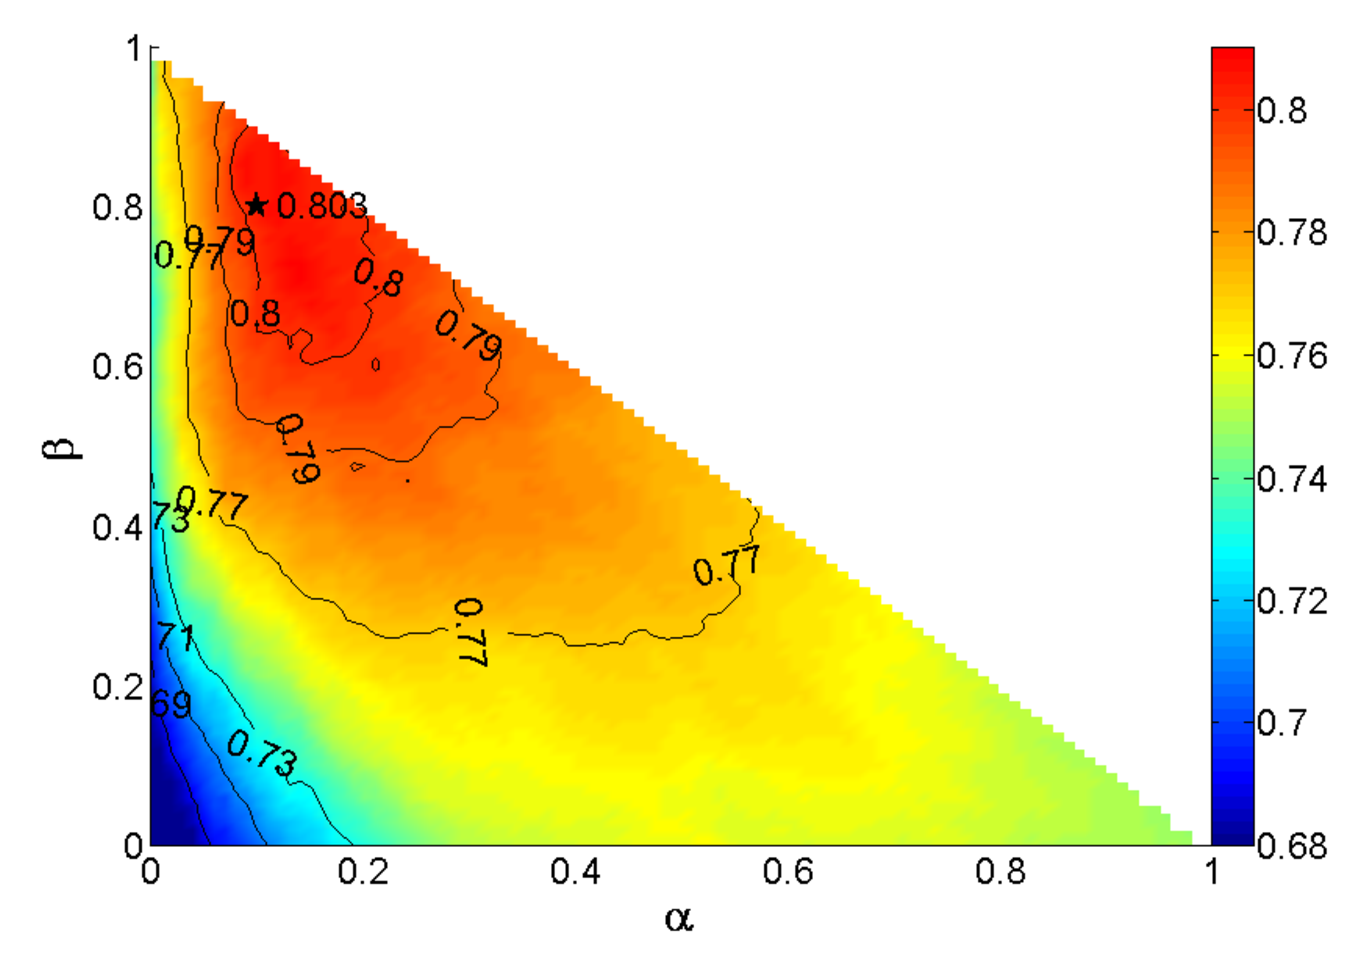
\includegraphics[scale=\graphscaleexpapp]{./exp/AAN-para-recm.eps}}
%\quad\quad
%\hspace{\graphmarginexpapp}
\hfill
\subfigure[{\scriptsize \aminer with \recom}]{\label{exp-aminer-ab-recom}
\includegraphics[scale=\graphscaleexpapp]{./exp/AMiner-para-recm.eps}}
%\quad\quad
%\hspace{\graphmarginexpapp}
\hfill
\subfigure[{\scriptsize \magdata with \recom}]{\label{exp-mag-ab-recom}
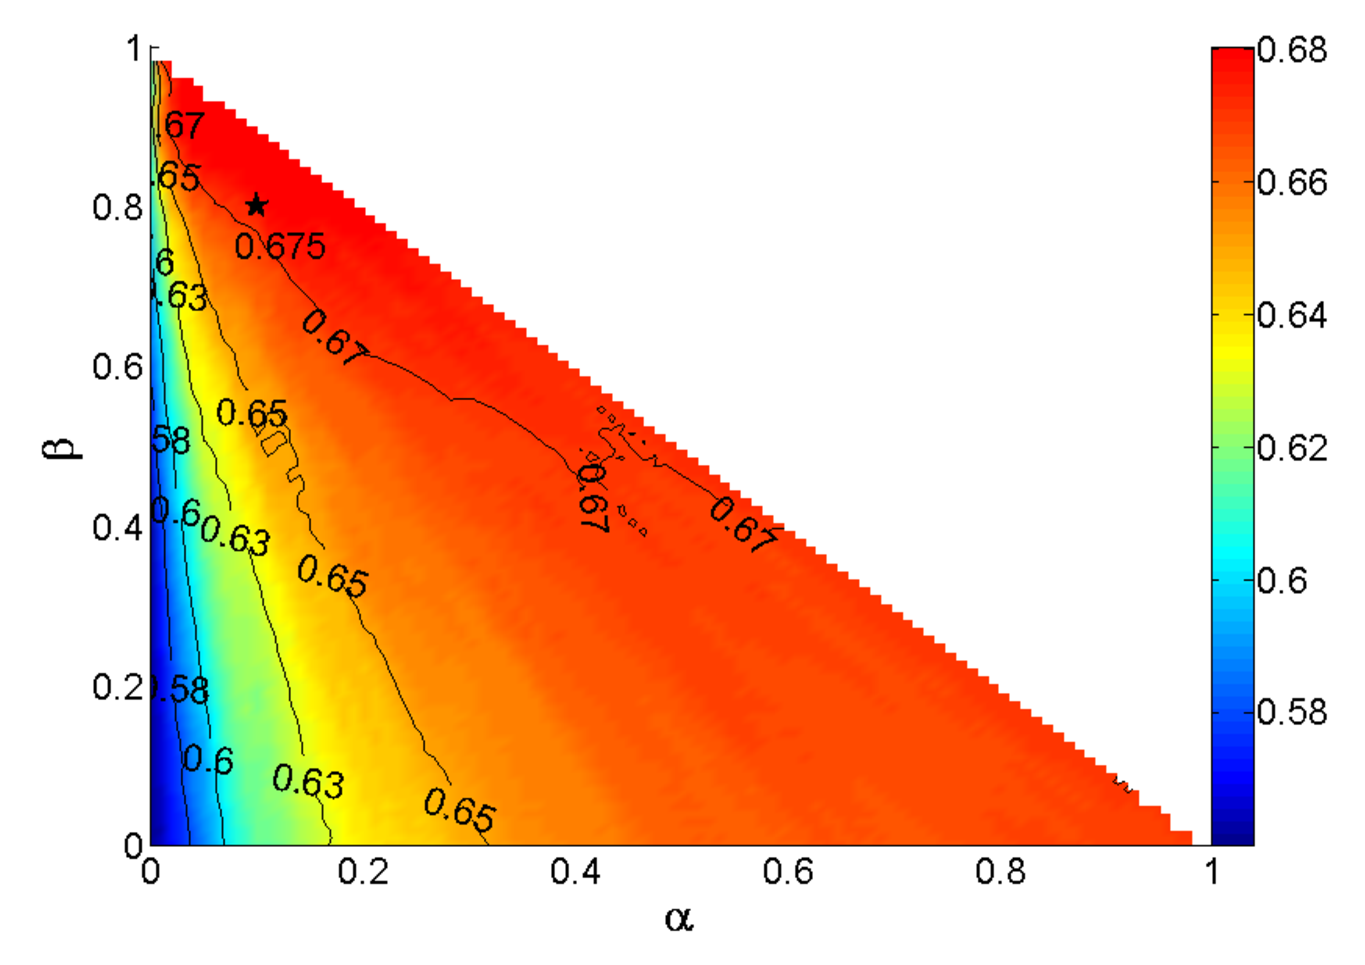
\includegraphics[scale=\graphscaleexpapp]{./exp/MAG-para-recm.eps}}
\\ %%%%%%%%%%%%%%%%%%%%%%%%%%%%%%%%%%%%%%
\vspace{-2ex}
%\hspace{-10ex}
\subfigure[{\scriptsize \aan  with \fcita}]{\label{exp-aan-ab-fcita}
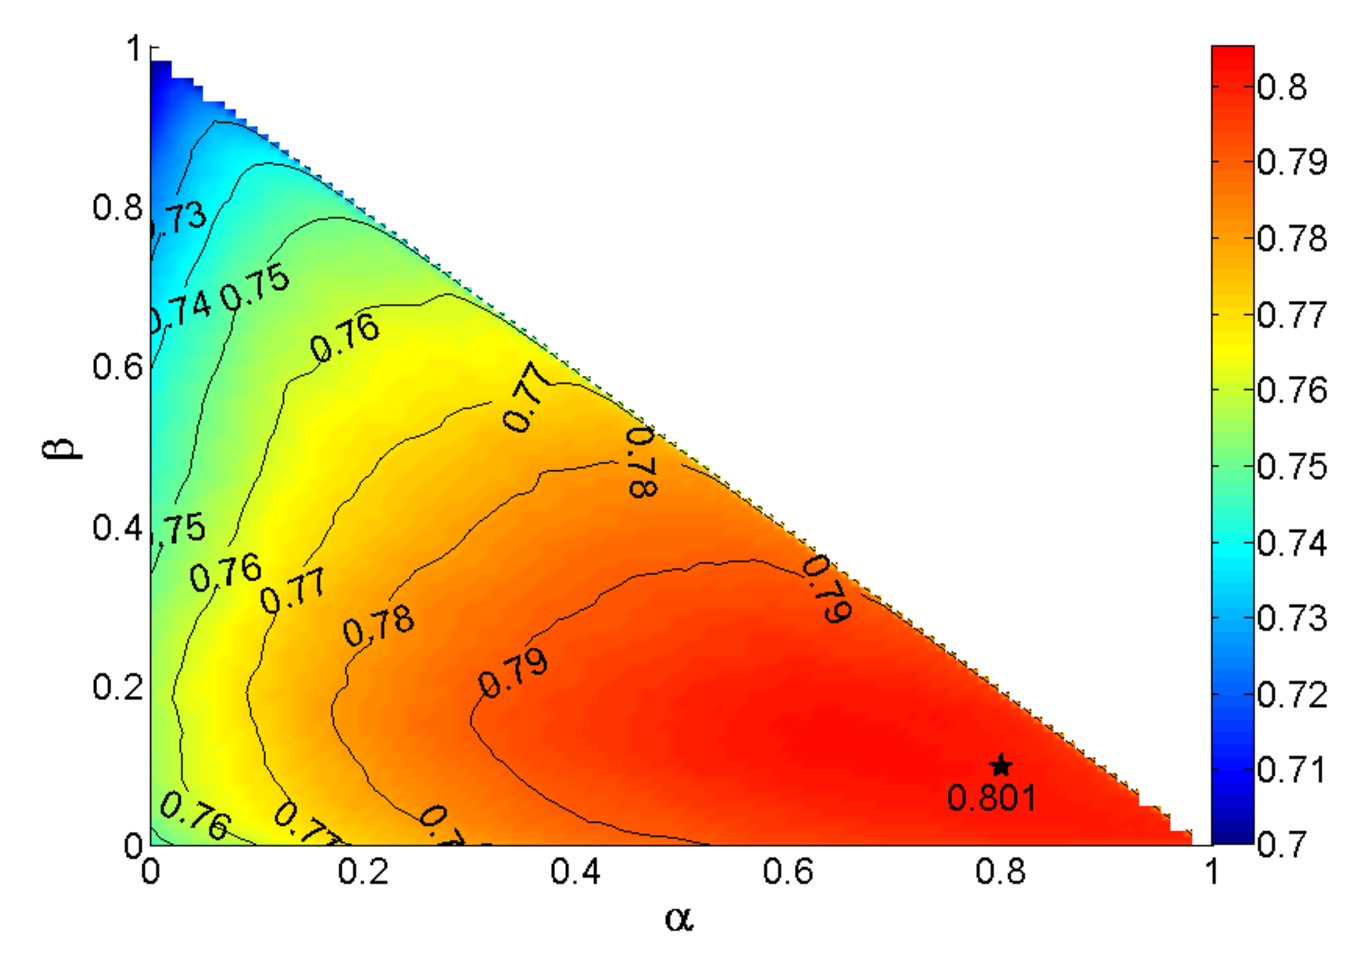
\includegraphics[scale=\graphscaleexpapp]{./exp/AAN-para-fcita.eps}}
%\quad\quad
%\hspace{\graphmarginexpapp}
\hfill
\subfigure[{\scriptsize \aminer with \fcita}]{\label{exp-aminer-ab-fcita}
\includegraphics[scale=\graphscaleexpapp]{./exp/AMiner-para-fcita.eps}}
%\quad\quad
%\hspace{\graphmarginexpapp}
\hfill
\subfigure[{\scriptsize \magdata with \fcita}]{\label{exp-mag-ab-fcita}
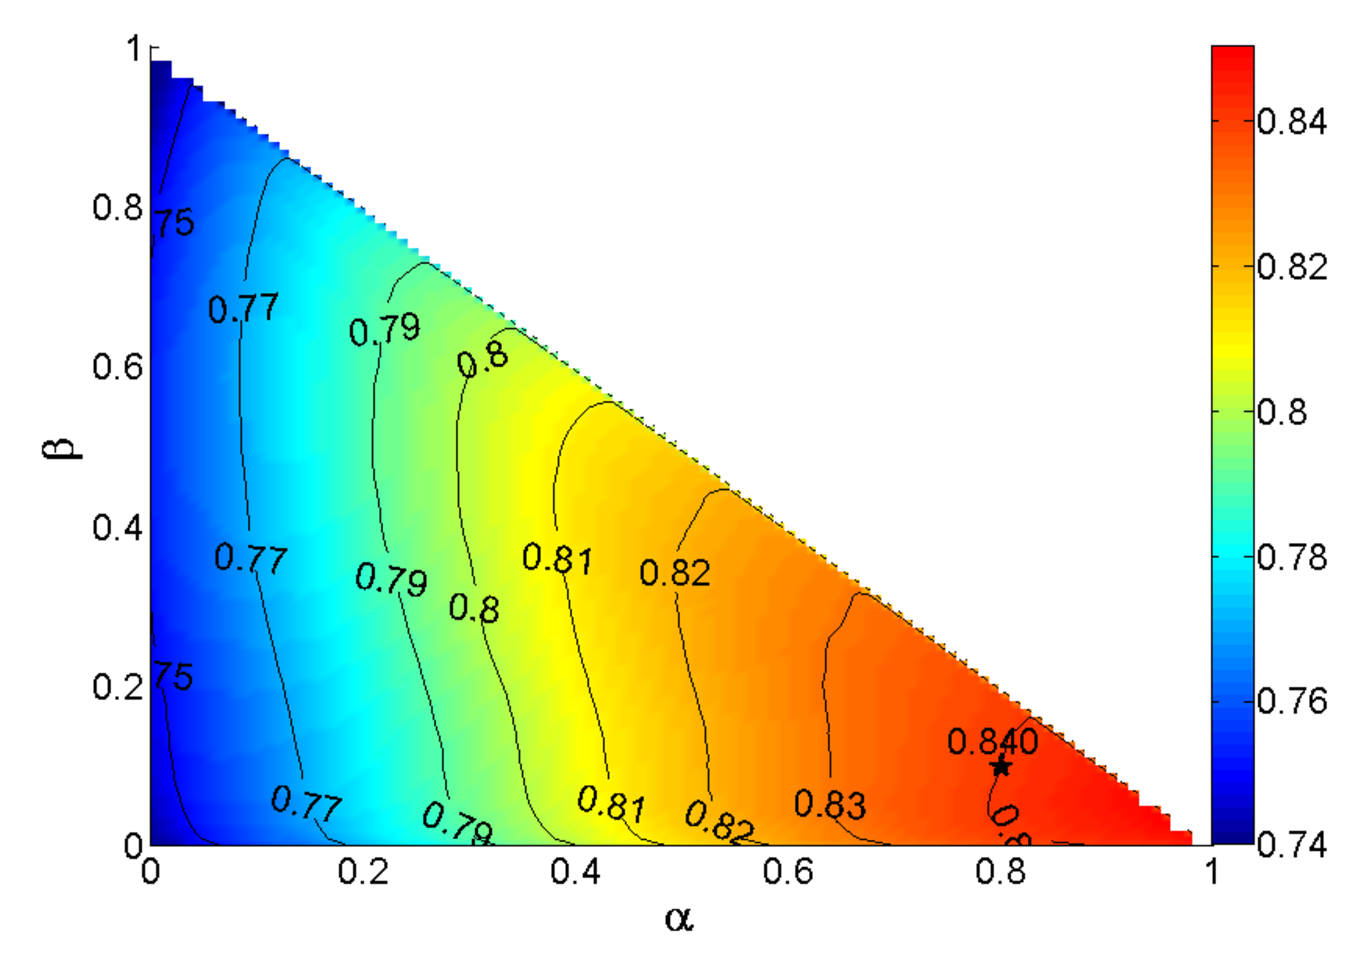
\includegraphics[scale=\graphscaleexpapp]{./exp/MAG-para-fcita.eps}}
\end{center}
\vspace{-2.5ex}
\caption{\small Accuracy tests: varying aggregating parameters $\alpha$ and $\beta$}
\label{exp-ab}
\vspace{-3ex}
\end{figure*}
%%%%%%%%%%%%%%%%%%%%%%%%%%%%%%%%%%%%%%

\stitle{Exp-4: Impacts of parameters}.
%\subsubsection{Exp-4: Impacts of parameters}.
In the last set of tests, we evaluated the impacts of time decaying factor $\sigma$, importance weighting factor $\lambda$, aggregating parameters $\alpha$ and $\beta$, and the TWPageRank. We fixed these parameters as well as $Y_s$ to their default values, used the TWPageRank proposed in this work by default, and tested the \PairAcc with the entire \recom and \fcita (\ie $T_i=+\infty$, $dif=1$).

%We present main results only and more details are available in~\cite{SARank-full}.




\etitle{Exp-4.1}.
%\stitle{Exp-4.1}.
To evaluate the impacts of the time decaying factor $\sigma$, we varied $\sigma$ from -1.6 to -0.4.
%, while fixed $Y_s$ to default values, $T_i=+\infty$, $dif=1$ and $\lambda=0.5$.
The results of \PairAcc are reported in Figs.~\ref{exp-aan-sigma}, \ref{exp-aminer-sigma} and \ref{exp-mag-sigma}.
%with both sets of ground-truth


When varying $\sigma$, the \PairAcc of \ensemblerank is very stable on all datasets using both \recom and \fcita. Indeed, with \recom and \fcita, the \PairAcc only varies (0.42\%, 1.55\%, 0.81\%) and (1.26\%, 0.96\%, 1.16\%) on (\aan, \aminer, \magdata), respectively.
%
%We omitted the detailed results of running time due to space constraint.
The running time varies (11.3\%, 8.6\%) on average only on (\aminer, \magdata), respectively.
%(0.18, 33.6) seconds, \ie

%Both of these show the robustness of \ensemblerank to the time decaying factor $\sigma$.

%As we can see from the figure, our method \ensemblerank is almost stable with the reduction of $\sigma$, since there is only a small fluctuation and the accuracy of our methods is always higher than the best baseline result in all datasets regardless of the change of $\sigma$. This means \ensemblerank is insensitive with $\sigma$.


%%%%%%%%%%%%%%%%%%%%%%%%%%%%%%%%%%%%%%%%%%%%%%%%%%
\begin{table}[tb!]
%\vspace{-2ex}
\begin{center}
\caption{\small Accuracy tests using different components with \recom (rows 2--4) and \fcita (rows 5--7).}
\label{tab-recom}
\begin{small}
\vspace{-.5ex}
\begin{tabular}{|c| c |c | c|}
\hline
{\bf Datasets} & {\bf C}\hspace{5ex}{\bf V}\hspace{5ex}{\bf A} & {\bf CV}\hspace{3ex}{\bf CA}\hspace{3ex}{\bf VA} & {\bf CVA} \\
\hline \hline
% \recom
\aan & 0.752 \ 0.616 \ 0.649 & 0.809 \ 0.764 \ 0.747 & {\bf 0.810} \\
\aminer & 0.735 \  0.581 \  0.640 & 0.784 \ 0.749 \ 0.729 & {\bf 0.785} \\
\magdata & 0.635 \ 0.534 \ 0.553 & 0.697 \ 0.673 \  0.648 & {\bf 0.698} \\ \hline
% \ficta
\aan & 0.785 \ 0.557 \ 0.761 & 0.849 \ 0.866 \ 0.771 & {\bf 0.870} \\
\aminer & 0.713 \  0.603 \  0.725 & 0.843 \ 0.847 \ 0.740 & {\bf 0.856} \\
\magdata & 0.736 \ 0.628 \ 0.718 & 0.848 \ 0.857 \ 0.751 & {\bf 0.874} \\
\hline
\end{tabular}
\end{small}
\end{center}
\vspace{-6ex}
\end{table}
%%%%%%%%%%%%%%%%%%%


\etitle{Exp-4.2}.
%\stitle{Exp-4.2}.
To evaluate the impacts of importance weighting factor $\lambda$, we varied $\lambda$ from 0 to 1.
%while fixed $Y_s$ to default values, $T_i=+\infty$, $dif=1$ and $\sigma=-1.0$.
The results of \PairAcc are reported in Figs.~\ref{exp-aan-lambda}, \ref{exp-aminer-lambda} and \ref{exp-mag-lambda}. Note that parameter $\lambda$ has no impacts on efficiency.
%with both sets of ground-truth

When varying $\lambda$, the \PairAcc of \ensemblerank first increases and then decreases on all datasets with both \fcita and \recom, except on \aminer with \recom.
%\marked{The value of $\lambda$ for \ensemblerank to achieve the best effectiveness is (0.6, 0, 0.2) and (0.6, 0.4, 0.1) on (\aan, \aminer, \magdata) with \recom and \fcita, respectively.}
This result indicates that combining prestige and popularity generally produces more robust results than using either of prestige and popularity.
Indeed, with \recom and \fcita, the \PairAcc of combining prestige and popularity is (10.2\%, 10.7\%, 5.5\%) and (8.0\%, 8.7\%, 9.0\%) higher than using prestige alone, and is (1.2\%, -0.1\%, 1.0\%) and (1.0\%, 1.0\%, 0.3\%) higher than using popularity alone on (\aan, \aminer, \magdata), respectively.


%The selection of $\lambda$ is influenced by ground-truth, such that the best $\lambda$ falls into $[xx,xx]$ and $[yy,yy]$ on \fcita and \recom, respectively. Moreover, equally weighting, \ie $\lambda=0.5$, is a good default setting when no query information is available in advance.
%Indeed, the best obtained \PairAcc using (\fcita, \recom) is only (0.10\%, 0.38\%), (0.04\%, 2.59\%) and (0.06\%, 0.91\%)  higher than the \PairAcc of equally weighting on \aan, \aminer and \magdata, respectively.





\etitle{Exp-4.3}.
To evaluate the impacts of aggregating parameters $\alpha$ and $\beta$, we varied $\alpha$ and $\beta$ at the granularity of 0.01. Again, parameters $\alpha$ and $\beta$ have few impacts on efficiency. The results are reported in Fig.~\ref{exp-ab}, where the parameters selected earlier and their corresponding \PairAcc are marked with $*$.

When varying $\alpha$ and $\beta$, the \PairAcc of \ensemblerank changes gently, as shown in Fig.~\ref{exp-ab}.
The optimal \PairAcc is obtained within a single region, rather than a complex collection of optimal regions.
%
Moreover, the \PairAcc keeps at a high level within a certain ($\alpha$, $\beta$) combination space around the optimal region, as shown in Fig.~\ref{exp-ab}.
%For instance, consider a square of length 0.3, which covers 8.5\% of the parameter combination space. The fraction of parameters such that the \PairAcc is no worse than 1\% of the corresponding \PairAcc with marker $*$ is (73\%, 94\%) on \aan, (96\%, 87\%) on \aminer and (83\%, 95\%) on \magdata, using (\recom, \fcita), respectively.
%
Further, the optimal parameters on the same sets of ground-truth are very similar for (\aan, \aminer and \magdata), indicating that the setting of $\alpha$ and $\beta$ can be easily transferred across different datasets.
To conclude, \ensemblerank is very robust to parameters $\alpha$ and $\beta$, and it is quite flexible for choosing proper values of parameters $\alpha$ and $\beta$.

Moreover, this enables to verify the effectiveness of importance assembling from different components, whose results are reported in Table~IV, in which letters C, V and A stand for citation, venue and author components, respectively.
The ranking based on all components consistently performs the best, using both \recom and \fcita, which justifies the use of importance assembling for ranking scholarly articles.
%which, using \recom and \fcita, improves the \PairAcc over using components (C, V, A, CV, CA, VA) by (5.77\%, 19.4\%, 16.1\%, 0.09\%, 4.59\%, 6.28\%) and (9.54\%, 23.7\%, 5.90\%, 2.50\%, 0.71\%, 4.79\%) on \aan, (6.94\%, 23.7\%, 14.4\%, 0.21\%, 1.56\%, 7.67\%) and (17.68\%, 12.4\%, 9.61\%, 0.33\%, 1.88\%, 6.34\%) on \aminer, and (6.29\%, 16.38\%, 14.45\%, 0.05\%, 2.43\%, 5.02\%) and (11.43\%, 19.2\%, 11.2\%, 1.44\%, 0.77\%, 9.62\%) on \magdata, respectively.


\eat{
\etitle{Exp-4.3}.
%\stitle{Exp-4.3}.
To evaluate the impacts of aggregating parameters $\alpha$ and $\beta$, we varied $\alpha$ and $\beta$ at the granularity of 0.01.
%while fixed $Y_s$ to default values, $T_i=+\infty$, $dif=1$, $\sigma=-1.0$ and $\lambda=0.5$.
Again, parameters $\alpha$ and $\beta$ have few impacts on efficiency. Due to space limitations, we only present the main results and more details are available at~\cite{SARank-full}.

Indeed, \ensemblerank is very robust to parameters $\alpha$ and $\beta$.
(a) When varying $\alpha$ and $\beta$, the \PairAcc of \ensemblerank changes gently. (b) \PairAcc also keeps at a high level within a certain ($\alpha$, $\beta$)  combination space. Finally, (c) the optimal parameters on the same set of ground-truth are very similar for \aan, \aminer and \magdata. That is, it is quite flexible for choosing proper values
of  parameters $\alpha$ and $\beta$.
} %%%%%%%% brief version of Exp-4.3

%%%%%%%%%%%%%%%%%%%%%%%%%%%%%%%%%%%%%%
\begin{figure*}[tb!]
%\vspace{1ex}
\addtolength{\subfigcapskip}{-1ex}
\begin{center}
\subfigure[{\scriptsize \aan with \recom}]{\label{exp-aan-recom-drank}
\includegraphics[scale=0.35]{./exp/AAN_TWPageRank_recom.eps}}
\hfill
%\hspace{\graphmarginexpapp}
\subfigure[{\scriptsize \aminer with \recom}]{\label{exp-aminer-recom-drank}
\includegraphics[scale=0.35]{./exp/AMiner_TWPageRank_recom.eps}}
\hfill
%\hspace{\graphmarginexpapp}
\subfigure[{\scriptsize \magdata with \recom}]{\label{exp-mag-recom-drank}
\includegraphics[scale=0.35]{./exp/MAG_TWPageRank_recom.eps}}
\\%%%%%%%%%%%%%%%%%%%%%%%%%%%%%%%%%%%%%%%%%%%
\vspace{-1.5ex}
\subfigure[{\scriptsize \aan with \fcita}]{\label{exp-aan-fcita-drank}
\includegraphics[scale=0.35]{./exp/AAN_TWPageRank_fcita.eps}}
\hfill
%\hspace{\graphmarginexpapp}
\subfigure[{\scriptsize \aminer with \fcita}]{\label{exp-aminer-fcita-drank}
\includegraphics[scale=0.35]{./exp/AMiner_TWPageRank_fcita.eps}}
\hfill
%\hspace{\graphmarginexpapp}
\subfigure[{\scriptsize \magdata with \fcita}]{\label{exp-mag-fcita-drank}
\includegraphics[scale=0.35]{./exp/MAG_TWPageRank_fcita.eps}}
\end{center}
\vspace{-2.5ex}
\caption{\small Impacts of the TWPageRank on accuracy: varying importance weighting
factor $\lambda$}
\label{exp-drank}
\vspace{-3ex}
\end{figure*}
%%%%%%%%%%%%%%%%%%%%%%%%%%%%%%%%%%

\newcommand{\drank}{\kw{DRank}}


\etitle{Exp-4.4}.
\marked{To evaluate the impacts of the proposed TWPageRank, we compared our approach \ensemblerank with an algorithm alternative (referred to as \drank) the same to \ensemblerank except exploiting exponentially decayed impact weights, \ie $w(u,v)=e^{\sigma(T_u-T_v)}$ in Eq.~(\ref{eq-infl-weights}).
%The two algorithms produce the same popularity while different prestige.
To better understand the impacts, we varied the importance weighting factor $\lambda$ from 0.1 to 1. Note that the ranking results are the same when $\lambda=0$ due to the same popularity computation. The results are reported in Fig.~\ref{exp-drank}, where the numbers represent the improvement of \PairAcc by \ensemblerank over the one by \drank.}

\marked{
When varying $\lambda$, the \PairAcc of \ensemblerank is better than the one of \drank in most cases, which shows the superiority of the TWPageRank than exploiting exponentially decayed weights.
The difference of \PairAcc by the two algorithms is higher with \recom than with \fcita, since the two algorithms are using citation information to predict past and future citations with \fcita.
Moreover, algorithm \ensemblerank is consistently better than \drank when $0.5 \le \lambda \le 0.9$.
%, which, with \recom and \fcita, improves the \PairAcc by (2.88\%, 3.91\%, 3.90\%) and (0.55\%, 0.50\%, 0.22\%) on (\aan, \aminer, \magdata) on average, respectively.
The improvement decreases with the decrease of $\lambda$ as the popularity dominates the ranking with small $\lambda$, and in some cases, \drank outperforms \ensemblerank. %as the prestige and popularity orders of article pairs are more diverse for \drank than \ensemblerank.
Overall, with \recom and \fcita, \ensemblerank improves the \PairAcc over \drank by (1.78\%, 3.07\%, 3.20\%) and (0.29\%, 0.48\%, 0.11\%) on (\aan, \aminer, \magdata) on average, respectively.
}

\marked{
The TWPageRank has little impacts on efficiency, and the running time of the two algorithms only varies (6.34\%, 4.83\%) on (\aminer, \magdata) on average, respectively.}

\eat{
With the increment of $\lambda$, \ensemblerank has more promotion than DRank and the \PairAcc of DRank is better than \ensemblerank with small $\lambda$, possibly due to the addition of popularity will correct the mistaken pairs better on DRank, although \ensemblerank rank more pairs correctly.
In addition, the change of \PairAcc with \recom is higher than the one with \fcita, possibly due to the article pairs in \fcita are of the same years.
Moreover, the \PairAcc of \ensemblerank is better than its counterparts from $\lambda=0.5$ to $\lambda=1$, except on \aminer with \fcita. Recall that in Fig.~\ref{exp-aminer-lambda} using popularity alone gives the best results on \aminer, indicating that the prestige computed by TWPageRank is less accurate on \aminer than on the other two datasets.
%
Indeed, with \recom and \fcita, the \PairAcc of \ensemblerank is (2.20\%, 6.63\%, 5.68\%) and (0.25\%, 0.05\%, 0.05\%) higher than DRank on (\aan, \aminer, \magdata), respectively, when using prestige alone, and is (1.73\%, 2.97\%, 2.92\%) and (0.22\%, -0.08\%, 0.17\%) higher when combining prestige and popularity, respectively, on average.
%
Finally, the TWPageRank has little impacts on efficiency, and the running time of \ensemblerank and its counterparts only changes (6.34\%, 4.83\%) on (\aminer, \magdata) on average, respectively.
}

\stitle{Summary}.
From these tests we find the followings.


\sstab(1) Our model \ensemblerank is effective for ranking scholarly articles, which is consistently better than competitive methods in all tests. With \recom and \fcita, \ensemblerank improves \PairAcc over (\pagerank, \futurerank, \hhgrank) by
(13.5\%, 6.8\%, 4.8\%) and (12.0\%, 3.0\%, 3.2\%) on \aan,
(12.7\%, 5.0\%, 4.9\%) and (14.0\%, 6.5\%, 4.6\%) on \aminer, and
(6.5\%, 2.5\%, 2.2\%) and (13.4\%, 6.0\%, 2.4\%) on \magdata, on average, respectively.
%, and it has a great advantage in evaluating the importance in a long term. Furthermore, it is more accurate evaluating articles which have just published and is in lack of citations, since it uses both venue network and author information besides of citation network. Indeed, it improves the accuracy by $(7.9\%, 3.2\%, 2.3\%)$ and $(14.4\%, 5.0\%, 3.8\%)$ over \pagerank, \futurerank and \hhgrank on average of three datasets with recommendation based ground truth and future citation ground truth, respectively.


\sstab(2) Our batch algorithm \batensemble and incremental algorithm \incensemble are also efficient.
%
Our incremental algorithm \incensemble is on average (1.7, 3.1, 2.8, 117) and (2.0, 3.0, 4.4, 245) times faster than (\batensemble, \powensemble, \futurerank, \hhgrank)  on the large \aminer and \magdata, respectively.

%The batch algorithm \batensemble is on average (1.3, 2.5, 348) times faster than (\powensemble, \futurerank, \hhgrank)  on the largest \magdata, respectively.

%\noindent (3) Our incremental algorithms are much faster than their batch counterparts in practice, even their time complexity is very close. Indeed, algorithms \inctwprdag, \inctwprscc and \incensemble further improve the efficiency of (\twprdag, \twprscc, \batensemble) by (23\%, 38\%, 22\%) on average, respectively.


\sstab(3) Our ranking model \ensemblerank introduces the time decaying factor $\sigma$, importance weighting factor $\lambda$ and aggregating parameters $\alpha$ and $\beta$ for the sake of practicability and flexibility in real-life applications, and, from our tests, \ensemblerank is very robust to these parameters. Moreover, the proposed TWPageRank is generally more effective than directly using exponentially decayed impact weights.




\stitle{Related work}. We summarize related work as follows.
%
%Scholarly article ranking

Scholarly article ranking has shifted from citation count analysis~\cite{Garfield471,Hirsch15112005} to graph analysis~\cite{ChenXMR07,Zhou07-CoRank,Jiang12-MRank,Liang16AAAI,Li08TSRanking,Wang13AAAI,WalkerXKM07,sayyadi09,
Wang16TIST,Ng11KDD}.
Based on the information used, these methods are divided into four categories: (a) using the citation information only~\cite{Garfield471,Hirsch15112005,ChenXMR07,Ng11KDD}, (b) using the citation and temporal information~\cite{Li08TSRanking,WalkerXKM07}, (c) using the citation information and other heterogeneous information, \eg authors and venues of articles~\cite{Zhou07-CoRank,Jiang12-MRank,Liang16AAAI}, and (d) combining the citation, temporal and other heterogeneous information~\cite{sayyadi09,Wang16TIST,Wang13AAAI}.
Our work belongs to the last category aiming at fully employing information available for scholarly article ranking.


%\stitle{PageRank\&weighted PageRank algorithms}.

%PageRank \cite{Brin98:PageRank} and its extensions have been extensively used for citation analyses \cite{Waltman2014}. While PageRank equally propagates scores along outlinks, Weighted PageRank \cite{Xing04:WPR} extends PageRank by distributing scores based on the popularity of pages. Different from previous work, the Time-Weighted PageRank proposed in this work discriminately propagates scores in terms of citation statistics.

PageRank \cite{Brin98:PageRank} and its extensions have been extensively used for citation analyses \cite{Waltman2014}. While PageRank equally propagates scores along outlinks, Weighted PageRank extends PageRank by distributing scores based on certain criteria such as popularity of pages~\cite{Xing04:WPR} or authority of authors~\cite{Ding11}. Different from previous work, the Time-Weighted PageRank proposed in this work discriminately propagates scores in terms of citation statistics.






%\stitle{Dynamic algorithms}.

Dynamic algorithms have proven useful for various tasks by avoiding computing from scratch~\cite{RamalingamR93}.
% and only recomputing those affected by updates
%Dynamic algorithms have proven useful for graph analysis tasks, \eg incremental graph pattern matching~\cite{FanWW13} and  incremental simrank computation~\cite{YuLZ14}.
To our knowledge, little concern has been paid to dynamic scholarly article ranking except that~\cite{GhoshKHLL11} uses PageRank in dynamic citation networks. However, its solution is based on a strong and impractical assumption that there are no citations between articles in the same years.
Further, although there exist several studies on incremental PageRank computation~\cite{DesikanPSK05,AbiteboulPC03,WuR09} and on incremental PageRank approximation \cite{BahmaniCG10,BahmaniKMU12}, they are not designed for scholarly article ranking.
%
Different from previous work, we study scholarly article ranking in a dynamic environment in terms of
the citation characteristics of scholarly articles, which has never been exploited before.

%Our approach only makes the assumption that there are no mutual references within the citation network, which, we admit, violates xx\% of total citations on \magdata, and is significantly different (yy\% on \magdata) from~\cite{GhoshKHLL11}.  - move to Section 3

Ensemble methods use multiple learners to obtain better performance than could be obtained from a constituent learner alone~\cite{zhihua-book}.
%In this work, we leverage ensembles to produce better and robust results for scholarly article ranking~\cite{zhihua-book,wsdmcup,DuanAMHH16}.
In this work, we leverage  importance assembling  to produce better and robust results for scholarly article ranking~\cite{zhihua-book,wsdmcup,DuanAMHH16}.


\section{Conclusions and Future Work}
We have proposed an ensemble-enabled approach for top-$k$ link prediction, which scales up link prediction on very large social networks. \marked{We speed up the top-$k$ predictions when a threshold is available.}
By decomposing a large network into smaller pieces, the bagging methods are more scalable to large networks with over 15 million nodes and 1 billion edges. We develop three bagging methods that are designed in particular for link prediction, and our bagging methods also provide better accuracy and scalability. \marked{Furthermore, we reduce the network sizes of ensembles in the bagging without sacrificing prediction accuracy. }
Finally, we have experimentally verified that our ensemble-enabled approach is much more accurate and scalable than existing methods \Aa \cite{adamic} and \BIGCLAM \cite{yang-wsdm2013}.

A couple of topics need further investigation. First, we are to develop distributed approaches scalable on networks with billions of nodes, in a way similar to \marked{ \cite{NMF-www2010, yu2015}}.   Second, we are to study personalized recommendations using our link prediction approach.



% if have a single appendix:
%\appendix[Proof of the Zonklar Equations]
% or
%\appendix  % for no appendix heading
% do not use \section anymore after \appendix, only \section*
% is possibly needed

% use appendices with more than one appendix
% then use \section to start each appendix
% you must declare a \section before using any
% \subsection or using \label (\appendices by itself
% starts a section numbered zero.)



% use section* for acknowledgment
% The Computer Society usually uses the plural form
\section*{Acknowledgments}
This work is supported in part by  973 program ({\small No. 2014CB340300}), NSFC ({\small No. 61322207}) and Special Funds of Beijing Municipal Science \& Technology Commission. For any correspondence, please refer to Shuai Ma.








% trigger a \newpage just before the given reference
% number - used to balance the columns on the last page
% adjust value as needed - may need to be readjusted if
% the document is modified later
%\IEEEtriggeratref{8}
% The "triggered" command can be changed if desired:
%\IEEEtriggercmd{\enlargethispage{-5in}}

% references section

% can use a bibliography generated by BibTeX as a .bbl file
% BibTeX documentation can be easily obtained at:
% http://mirror.ctan.org/biblio/bibtex/contrib/doc/
% The IEEEtran BibTeX style support page is at:
% http://www.michaelshell.org/tex/ieeetran/bibtex/
%\bibliographystyle{IEEEtran}
% argument is your BibTeX string definitions and bibliography database(s)
%\bibliography{IEEEabrv,../bib/paper}
%
% <OR> manually copy in the resultant .bbl file
% set second argument of \begin to the number of references
% (used to reserve space for the reference number labels box)

\marked{
\begin{footnotesize}
\bibliographystyle{abbrv}
\bibliography{paper}
\end{footnotesize}}


\eat{

\begin{thebibliography}{1}

\bibitem{adamic}
L.~Adamic and E.~Adar. Friends and neighbors on the web. {\em
Social Networks}, 25, pp. 211--230, 2001.

\bibitem{conceptualr} C. Aggarwal and S. Parthasarathy. Mining
massively incomplete data sets by conceptual reconstruction. {\em
KDD}, 2001.

\bibitem{adom} G. Adomavicius, and A. Tuzhilin.
Toward the next generation of recommender systems: A survey of the
state-of-the-art
 and possible extensions. {\em IEEE Transactions on Knowledge and Data Engineering (TKDE)},
 17(6), pp. 734--749, 2005.

\bibitem{adafre}
S. F. Adafre and M.  Rijke. Discovering missing links in Wikipedia.
{\em KDD Workshop on Link Discovery}, 2005.


\bibitem{back} L. Backstrom, and J. Leskovec.
 Supervised random walks: predicting and recommending
 links in social networks. {\em WSDM}, 2011.

  \bibitem{bilgic}
M. Bilgic,  G. Namata and L. Getoor.  Combining collective
classification and link prediction. {\em ICDM Workshop on Mining
Graphs and Complex Structures}, 2007.


\bibitem{chancc}
L.~Getoor and C.~Diehl. Link mining: A survey.
{\em SIGKDD Exploration}, pp. 3--12, 2005.


\bibitem{Link09}
J.~R. Doppa, J.~Yu, P.~Tadepalli and L.~Getoor.
\newblock  Chance constrained programs for link prediction.
\newblock {\em NIPS Workshop on Analyzing Networks and Learning with Graphs},
2009.

\bibitem{menon} A. K. Menon, and C. Elkan.
Link prediction via matrix factorization. {\em Machine Learning and
Knowledge Discovery in Databases}, pp. 437--452, 2011.

\bibitem{Getoor01}
L.~Getoor, N.~Friedman, D.~Koller and B.~Taskar.
\newblock  Learning probabilistic models of relational
structure.
\newblock {\em ICML}, 2001.

\bibitem{Getoor02}
L.~Getoor, N.~Friedman, D.~Koller and B.~Taskar.
\newblock  Learning probabilistic models of link structure.
\newblock {\em Journal of Machine Learning Research}, 3, pp. 679--707, 2002.



%\bibitem{hopcroft} J. Hopcroft, T. Lou, and  J. Tang.
% Who will follow you back?: reciprocal relationship prediction.
%{\em  CIKM}, 2011.



\bibitem{kunegis}
J. Kunegis and A. Lommatzsch.  Learning Spectral Graph
Transformations for Link Prediction. {\em ICML}, 2009.



\bibitem{kleinberg}
D.~Liben-Nowell and J.~Kleinberg.
\newblock The link prediction problem for social networks.
\newblock {\em  Journal of the American society for information science and technology},
58(7), pp. 1019--1031, 2007.

\bibitem{long} B. Long, Z.  Zhang, and P. Yu. Co-clustering by block value decomposition.
{\em KDD}, 2005.


\bibitem{propflow} R. Lichtenwalter, J. Lussier, and N. Chawla. New perspectives and
methods in link prediction. {\em  KDD},  2010.


%\bibitem{lichen2} R.  Lichtenwalter and N.  Chawla.  Lpmade: Link
%prediction made easy. {\em Journal of Machine Learning Research},
%12: pp. 2489--2492, 2011.

\bibitem{lichen3} R. Lichenwater and N.  Chawla.
Vertex Collocation Profiles: Subgraph Counting for Link Analysis and
Prediction. {\em WWW}, 2012.

\bibitem{web} B. Liu. Web Data Mining. {\em Springer}, 2010.

\bibitem{qi} G.  Qi, C. Aggarwal, and T. Huang. Link Prediction
across Networks by Cross-Network Biased Sampling. {\em ICDE}, 2013.



\bibitem{sun11} Y. Sun, R. Barber, M. Gupta,  C. Aggarwal, J.
Han.  Co-author Relationship Prediction in Heterogeneous
Bibliographic Networks.  {\em ASONAM}, 2011.

\bibitem{sun12} Y. Sun, J. Han, C. Aggarwal, N. Chawla.  When will it
happen -- Relationship Prediction in Heterogeneous Information
Networks.  {\em WSDM}, 2012.


\bibitem{tang}   J. Tang, T. Lou,  and J. Kleinberg.
 Inferring social ties across heterogenous networks. {\em  WSDM}, 2012.


\bibitem{Taskar03}
B.~Taskar, M.~F. Wong, P.~Abbeel and D.~Koller.
\newblock  Link prediction in relational data.
\newblock {\em NIPS}, 2003.



\bibitem{dwang} D. Wang, D. Pedreschi, C. Song, F. Giannotti, and A.-L.
Barabasi.   Human mobility, social ties, and link prediction. {\em
KDD}, 2011.


\bibitem{yang} Y. Yang, N. Chawla, Y.  Sun, and J. Han. Predicting Links in
Multi-Relational and Heterogeneous Networks. {\em ICDM}, 2012.

\bibitem{Yang09}
T.~Yang, R.~Jin, Y.~Chi, and S.~Zhu.
  Combining link and content for community detection: a discriminative
  approach.
 {\em KDD}, 2009.

\bibitem{yu}
K. Yu, W. Chu,  S. Yu,  V.  Tresp and Z. Xu. Stochastic
relational models for discriminative link prediction. {\em NIPS}, 2006.



\bibitem{zhu}
J. Zhu, J. Hong and G. Hughes.  Using Markov models for web site
link prediction. {\em  HyperText}, 2002.


\bibitem{ding}
C. Ding, X. He and H. D. Simon. On the Equivalence of Nonnegative
Matrix Factorization and Spectral Clustering. {\em SDM}, 2005.

%\bibitem{berman}
%A. Berman, Complete Positivity, {\em Linear Algorithm and Its
%Applications}, 107:57---63, 1998.

\bibitem{lee}
C. Lee, M. Pham, N. Kim, M. K. Jeong, D. K. J. Lin and W. Art. A
Novel Link Prediction Approach for Scale-free Networks. {\em WWW}, 2014.

\bibitem{NMF-nature99}
Lee, Daniel D. and Seung, H. Sebastian. Learning the parts of objects by non-negative matrix factorization. {\em Nature},  401, pp. 788--791, 1999.

\bibitem{NMF-www2010}
Chao Liu, Hung-chih Yang, Jinliang Fan, Li-Wei He and Yi-Min Wang.
{Distributed Nonnegative Matrix Factorization for Web-Scale Dyadic Data Analysis on MapReduce}.
{\em WWW}, 2010.


\bibitem{ahmed2014tkdd}
Ahmed, Nesreen K. and Neville, Jennifer and Kompella, Ramana. Network Sampling: From Static to Streaming Graphs. {\em Transactions on Knowledge Discovery from Data (TKDD)}, 8(2), pp. 7:1--7:56 2014.

\bibitem{yang-wsdm2013}
Jaewon Yang and Jure Leskovec. Overlapping Community Detection at Scale: A Nonnegative Matrix
Factorization Approach. {\em WSDM}, 2013.

\bibitem{katz-1953}
L. Katz. A New Status Index Derived from Sociometric Analysis. {\em Psychometrika}, 18(1), pp. 39--43, 1953.

\bibitem{linyuan-2011}
Linyuan Lu and Tao Zhou. Link Prediction in Complex Networks: A Survey.
{\em Physica A}, pp. 1150--1170, 2011.

\bibitem{Hasan-2011}
Mohammad Al Hasan and Mohammed J. Zaki.
\newblock A survey of link prediction in social networks.
\newblock {\em Social Network Data Analytics}, 2011.

\bibitem{leskovec-2008}
J. Leskovec, L. Backstrom, R. Kumar and A. Tomkins. Microscopic Evolution of Social Networks.
{\em KDD}, 2008.

\bibitem{Breiman96b-1996}
Leo Breiman. Bagging Predictors. {\em Machine Learning},
24(2), pp. 123--140, 1996.

\bibitem{barbieri2014}
N. Barbieri, F. Bonchi and G. Manco. Who to Follow and Why: Link Prediction with Explanations.
{\em KDD}, 2014.

\bibitem{tang2015}
J. Tang, S. Chang, C. Aggarwal and H. Liu. Negative Link Prediction in Social Media.
{\em WSDM}, 2015.

\bibitem{west2015}
R. West, A. Paranjape and J. Leskovec. Mining Missing Hyperlinks from Human Navigation Traces:
A Case Study of Wikipedia. {\em WWW}, 2015.

\bibitem{liang2016}
L. Duan, C. Aggarwal, S. Ma, R. Hu and J. Huai. Scaling up Link Prediction with Ensembles.
{\em WSDM}, 2016.





\end{thebibliography}


}%%%%%%%%%%%% /eat


% biography section
%
% If you have an EPS/PDF photo (graphicx package needed) extra braces are
% needed around the contents of the optional argument to biography to prevent
% the LaTeX parser from getting confused when it sees the complicated
% \includegraphics command within an optional argument. (You could create
% your own custom macro containing the \includegraphics command to make things
% simpler here.)
%\begin{IEEEbiography}[{\includegraphics[width=1in,height=1.25in,clip,keepaspectratio]{mshell}}]{Michael Shell}
% or if you just want to reserve a space for a photo:

%IEEEbiography

\begin{IEEEbiography}{Liang Duan} is a PhD student in the School of Computer Science and Engineering, Beihang University, supervised by Prof. Shuai Ma. He received his MS degree in computer software and theory from Yunnan University in 2014, and BS degree in computer science and technology from Beihang University in 2009. His current research interests include databases and social data analysis.
\end{IEEEbiography}

\begin{IEEEbiography}{Charu Aggarwal} received the BS degree
from IIT Kanpur in 1993 and the PhD degree
from Massachusetts Institute of Technology in
1996. He is a research scientist at the IBM T.J.
Watson Research Center in Yorktown Heights,
New York. He has since worked in the field of
performance analysis, databases, and data mining.
He has published more than 155 papers in
refereed conferences and journals, and has been
granted over 50 patents. He has served on the
program committees of most major database/
data mining conferences, and served as program vice-chairs of the
SIAM Conference on Data Mining, 2007, the IEEE ICDM Conference,
2007, the WWW Conference 2009, and the IEEE ICDM Conference,
2009. He served as an associate editor of the IEEE Transactions on
Knowledge and Data Engineering Journal from 2004 to 2008. He is an
associate editor of the ACM TKDD Journal, an action editor of the Data
Mining and Knowledge Discovery Journal, an associate editor of the
ACM SIGKDD Explorations, and an associate editor of the Knowledge
and Information Systems Journal. He is a fellow of the IEEE for
��contributions to knowledge discovery and data mining technique��, and
a life member of the ACM.
\end{IEEEbiography}


\begin{IEEEbiography}{Shuai Ma} is a professor at the School of Computer Science and Engineering, Beihang University, China.
He obtained his PhD degrees from University of Edinburgh in 2010, and from
Peking University in 2004, respectively.
He was a postdoctoral research fellow in the database group, University of Edinburgh, a summer intern at Bell labs, Murray Hill, USA and a visiting researcher of MRSA.
He is a recipient of the best paper award for VLDB 2010 and the best challenge paper award for WISE 2013. His current research interests include database theory and systems, social data and graph analysis, and data intensive computing.
\end{IEEEbiography}
\vspace{-6ex}


%\begin{IEEEbiography}{Renjun Hu}
%Biography text here.
%\end{IEEEbiography}

\vspace{-6ex}
\begin{IEEEbiography}{Jinpeng Huai} is a professor at the School of Computer Science and Engineering, Beihang University, China. He received his Ph.D. degree in computer science from Beihang University, China, in 1993. Prof. Huai is an academician of Chinese Academy of Sciences and the vice honorary chairman of China Computer Federation (CCF). His research interests include big data computing, distributed systems, virtual computing, service-oriented computing, trustworthiness and security.
\end{IEEEbiography}




% that's all folks
\end{document}


